%%%%%%%%%%%%%%%%%%%%%%%%%%%%%%%%%%%%%%%%%%%%%%%%%%%%%%%%%%%%%%%%%%%%%%
% Overleaf (WriteLaTeX) Example: Molecular Chemistry Presentation
%
% Source: http://www.overleaf.com
%
% In these slides we show how Overleaf can be used with standard 
% chemistry packages to easily create professional presentations.
% 
% Feel free to distribute this example, but please keep the referral
% to overleaf.com
% 
%%%%%%%%%%%%%%%%%%%%%%%%%%%%%%%%%%%%%%%%%%%%%%%%%%%%%%%%%%%%%%%%%%%%%%

\documentclass[xcolor={dvipsnames}]{beamer}

\mode<presentation>
{
  \usetheme{Madrid}       % or try default, Darmstadt, Warsaw, ...
  \usecolortheme{default} % or try albatross, beaver, crane, ...
  \usefonttheme{default}    % or try default, structurebold, ...
  \setbeamertemplate{navigation symbols}{}
  \setbeamertemplate{caption}[numbered]
} 

\usepackage[english]{babel}
\usepackage[utf8x]{inputenc}
\usepackage{graphicx}
\usepackage{hyperref}
  \hypersetup{colorlinks=true}
  \hypersetup{urlcolor=blue}
  \hypersetup{linkcolor = .}
\usepackage{xcolor}
\usepackage{siunitx}
  \sisetup{separate-uncertainty = true}
\usepackage{physics}
\usepackage[font=small,labelfont=bf]{caption}
\usepackage{subcaption}
\usepackage[en-GB]{datetime2}
\usepackage{overpic}
\usepackage{feynmp}
\DeclareGraphicsRule{*}{mps}{*}{}
\usepackage{scalerel}
\newcommand{\mylbrace}[2]{\vspace{#2pt}\hspace{6pt}\scaleleftright[\dimexpr5pt+#1\dimexpr0.06pt]{\lbrace}{\rule[\dimexpr2pt-#1\dimexpr0.5pt]{-4pt}{#1pt}}{.}}
\newcommand{\myrbrace}[2]{\vspace{#2pt}\scaleleftright[\dimexpr5pt+#1\dimexpr0.06pt]{.}{\rule[\dimexpr2pt-#1\dimexpr0.5pt]{-4pt}{#1pt}}{\rbrace}\hspace{6pt}}

% Trim in percent
\usepackage{adjustbox}

% No "Figure" prefix
\setbeamertemplate{caption}{\raggedright\insertcaption\par}

% Nice decay amplitude diagrams
\usepackage{amsmath,amssymb,tikz-cd}

% Strike out text
\usepackage[normalem]{ulem}

% For figures with text overlay
\usepackage{overpic}

% Arrows
\usepackage{tikz}
\newcommand{\tikzmark}[1]{\tikz[remember picture] \node[coordinate] (#1) {#1};}

% Colourbox with line breaks
\newcommand{\cbox}[2][lime!20]{%
  \colorbox{#1}{\parbox{\dimexpr\linewidth-2\fboxsep}{\strut #2\strut}}%
}

% Vector arrows
\usepackage[pdftex]{pict2e}

% Here's where the presentation starts, with the info for the title slide
\title[LHCb-UK RAL]{TORCH test beam analysis and developments in MCP-PMTs and electronics}

\author[Martin Tat]{Martin Tat, on behalf of the TORCH collaboration}
\institute[University of Oxford]{\normalsize LHCb-UK annual meeting, RAL}
\date{8th-10th January 2024}

\titlegraphic{
\includegraphics[height = 1.3cm]{Logos/OxfordLogo.pdf}\hspace{0.5cm}~%
              
\includegraphics[height = 1.3cm]{Logos/Warwick_logo.png}\hspace{0.5cm}~%
              \includegraphics[height = 1.3cm]{Logos/Edinburgh_logo.png}\hspace{0.5cm}~%
              
\includegraphics[height = 1.3cm]{Logos/Jozef_Stefan_Institute_logo.jpg}\hspace{0.5cm}~%
              
\includegraphics[height = 1.3cm]{Logos/Bristol_logo.jpg}\hspace{2.5cm}~%
              
\includegraphics[height = 1.3cm]{Logos/CERNLogo.png}\hspace{0.5cm}~%
              
\includegraphics[height = 1.3cm]{Logos/Photek_logo.jpg}\hspace{0.5cm}~%
              
\includegraphics[height = 1.3cm]{Logos/lhcb.jpg}}

\begin{document}

\begin{frame}
  \titlepage
\end{frame}

% These three lines create an automatically generated table of contents.
% \begin{frame}{Outline}
%   \tableofcontents
% \end{frame}

\section{Introduction to TORCH}
\begin{frame}{Introduction to TORCH}
  \vspace{0.0cm}
  \begin{center}
    {\large TORCH: Time Of internally Reflected CHerenkov light}
  \end{center}
  \begin{itemize}
    \setlength\itemsep{0.3em}
    \item{Particle identification at LHCb at low momentum ($2$-$\SI{20}{\giga\eV}$)}
    \item{Ensure full coverage of LHCb's flavour physics programme}
    \begin{enumerate}
      \setlength\itemsep{0.3em}
      \item{Boost signal efficiencies and suppress mis-ID backgrounds}
      \item{Improve flavour tagging efficiency by $25$-$50\%$}
    \end{enumerate}
  \end{itemize}
  \begin{figure}
    \centering
    \begin{subfigure}{0.57\textwidth}
      \centering
      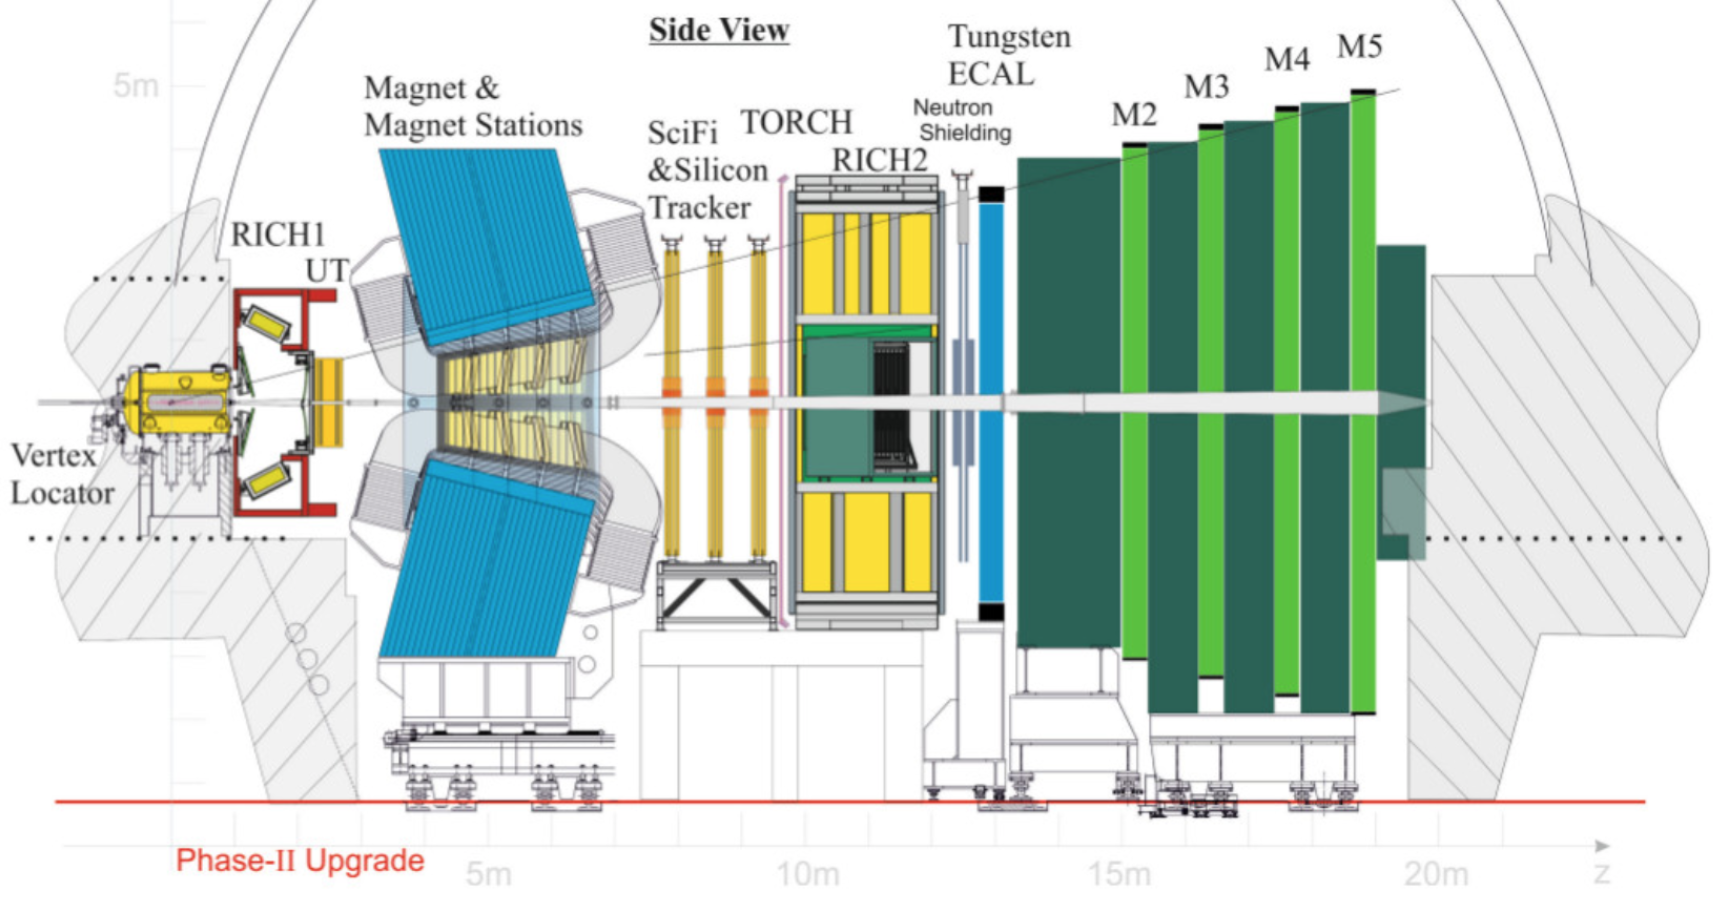
\includegraphics[width = 1.0\textwidth]{Figs/TORCH_location.png}
    \end{subfigure}%
    \begin{subfigure}{0.43\textwidth}
      \centering
      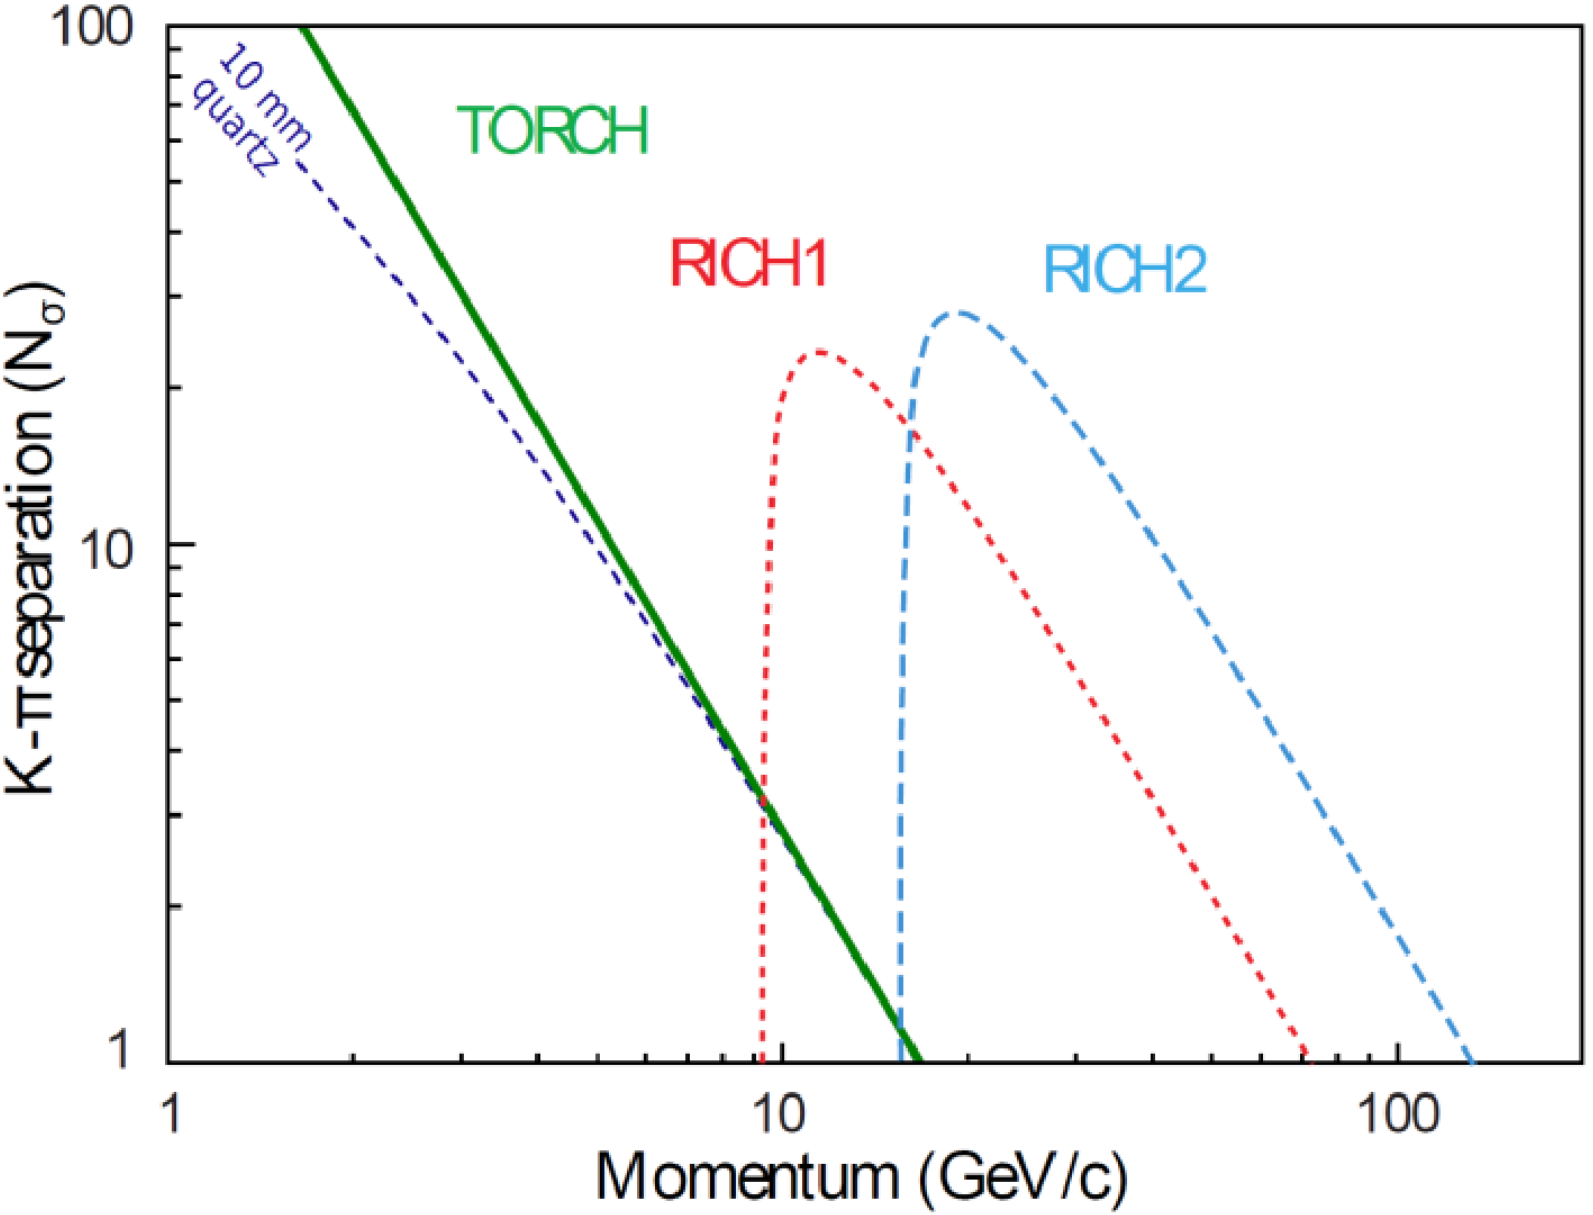
\includegraphics[width = 1.0\textwidth]{Figs/TORCH_RICH_separation.png}
    \end{subfigure}
  \end{figure}
\end{frame}

\begin{frame}{Introduction to TORCH}
  \vspace{0.0cm}
  \begin{center}
    {\large PID with Time-of-Flight, combined with Cherenkov information}
  \end{center}
  \begin{itemize}
    \item{Cover physics region inaccessible to RICH}
    \item{$\pi$-$K$ ToF difference over $\SI{10}{\meter}$ $\implies$ Aim for $10$-$\SI{15}{\pico\second}$ resolution}
    \item{Single-photon precision of $\SI{70}{\pico\second}$ with $\sim 30$ detected photons}
  \end{itemize}
  \begin{figure}
    \centering
    \begin{subfigure}{0.5\textwidth}
      \centering
      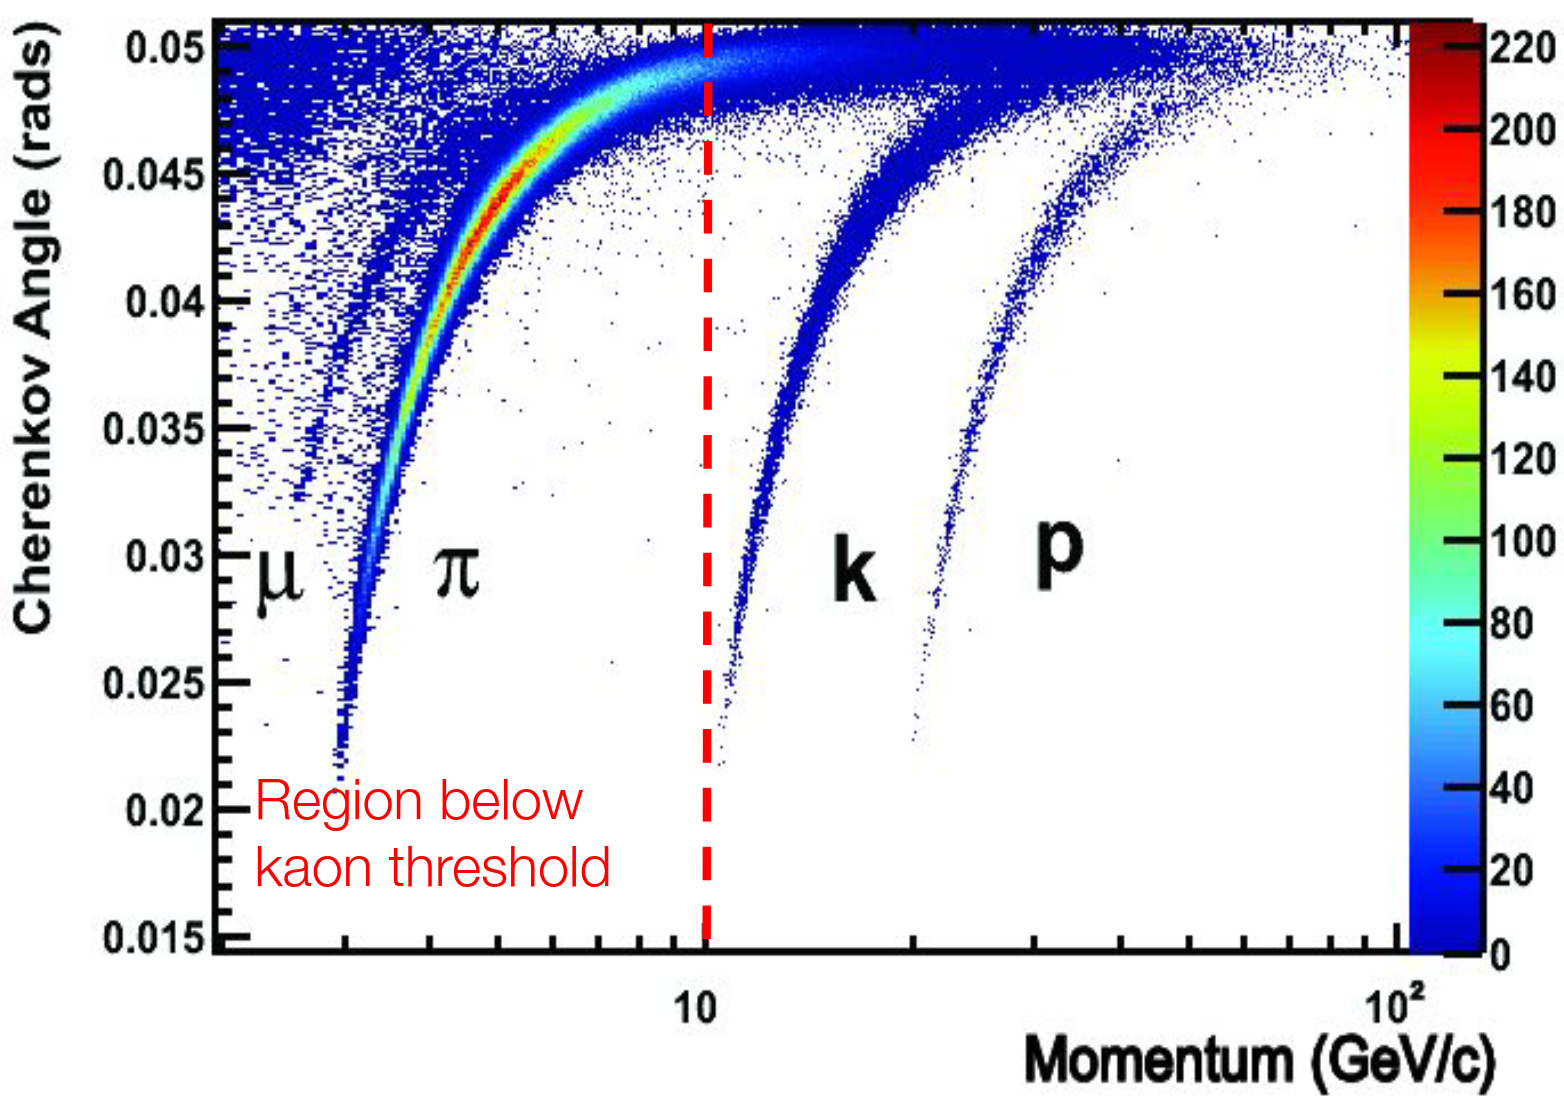
\includegraphics[width = 1.0\textwidth]{Figs/RICH_CherenkovAngle.png}
    \end{subfigure}%
    \begin{subfigure}{0.5\textwidth}
      \centering
      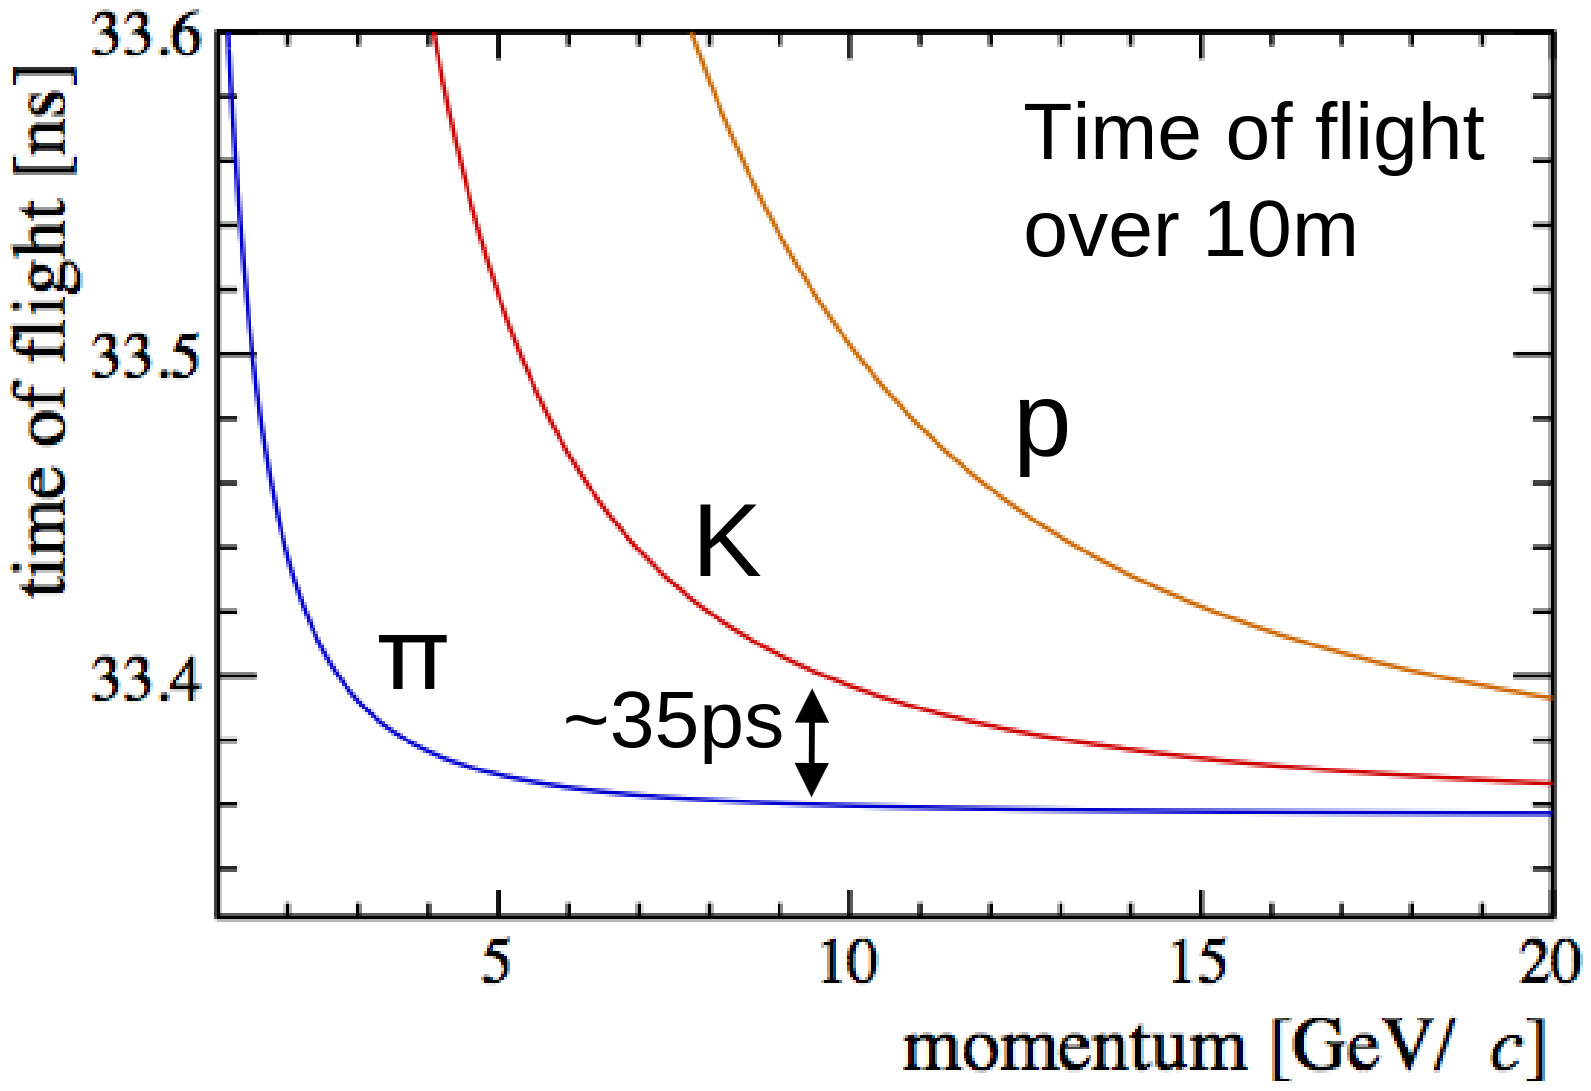
\includegraphics[width = 1.0\textwidth]{Figs/TORCH_ToF.png}
    \end{subfigure}
  \end{figure}
\end{frame}

\section{TORCH working principle}
\begin{frame}{TORCH working principle}
  \begin{columns}
    \begin{column}{0.55\textwidth}
      \begin{enumerate}
        \setlength\itemsep{1.5em}
        \item{Charged particle enter quartz}
        \item{Cherenkov photons emitted}
        \item{Photons undergo internal reflection until they reach the top of the plate}
      \end{enumerate}
      \begin{figure}
        \centering
        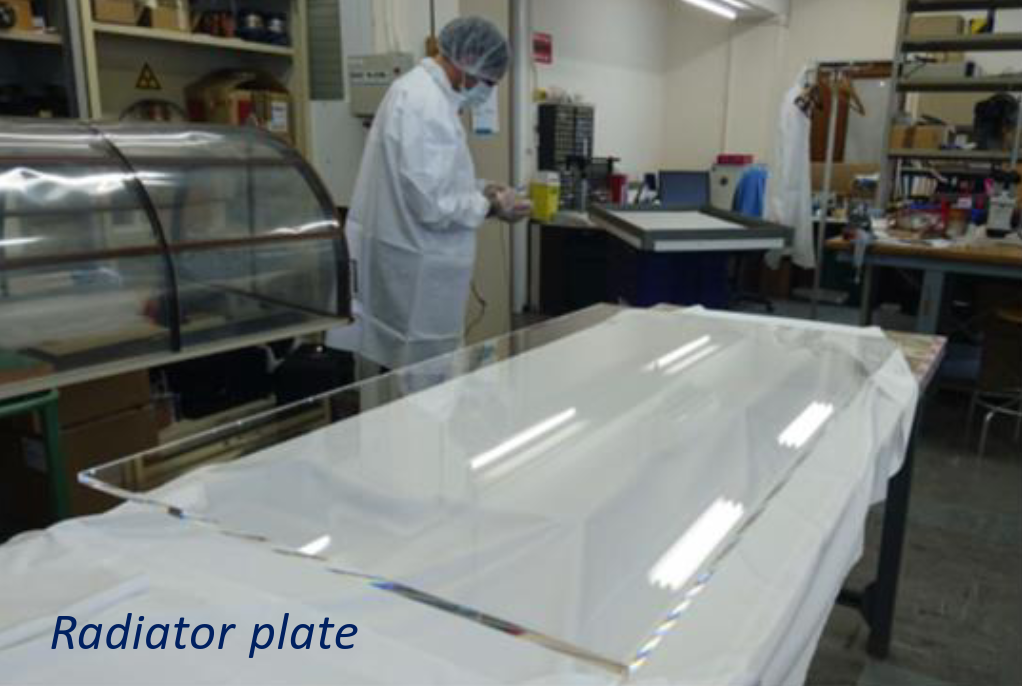
\includegraphics[width = 0.8\textwidth]{Figs/RadiatorPlate_lab.png}
      \end{figure}
    \end{column}
    \begin{column}{0.45\textwidth}
      \begin{figure}
        \centering
        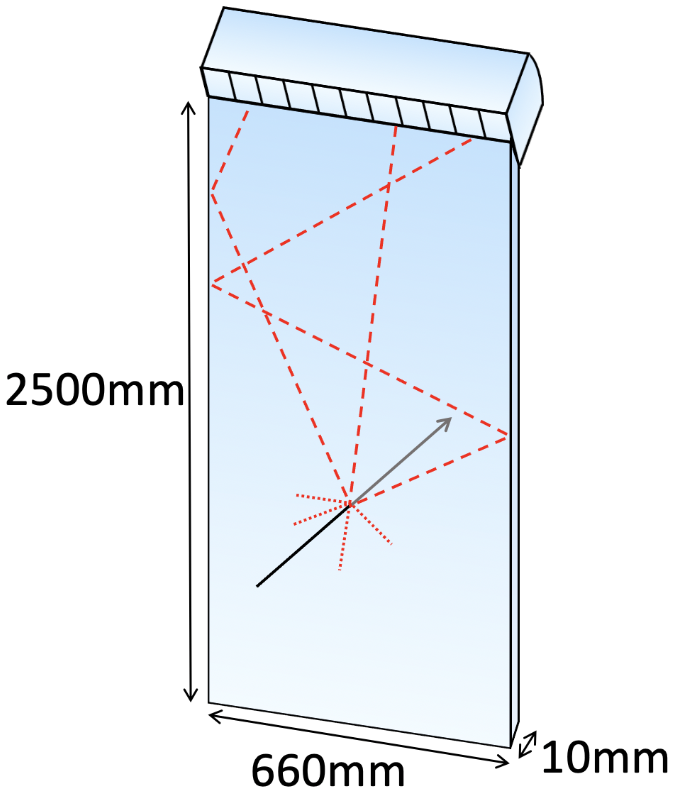
\includegraphics[width = 1.0\textwidth]{Figs/TORCH_FrontView.png}
      \end{figure}
    \end{column}
  \end{columns}
\end{frame}

\begin{frame}{TORCH working principle}
  \begin{columns}
    \begin{column}{0.65\textwidth}
      \begin{enumerate}
        \setlength\itemsep{1.0em}
        \item{Focus photons with cylindrical mirrror}
        \item{Image consists of hyperbolic ``bands''}
        \begin{itemize}
          \item{Compare with circular rings in RICH}
        \end{itemize}
        \item{Correct for chromatic dispersion using the Cherenkov angle obtained from $y'$}
      \end{enumerate}
      \begin{figure}
        \centering
        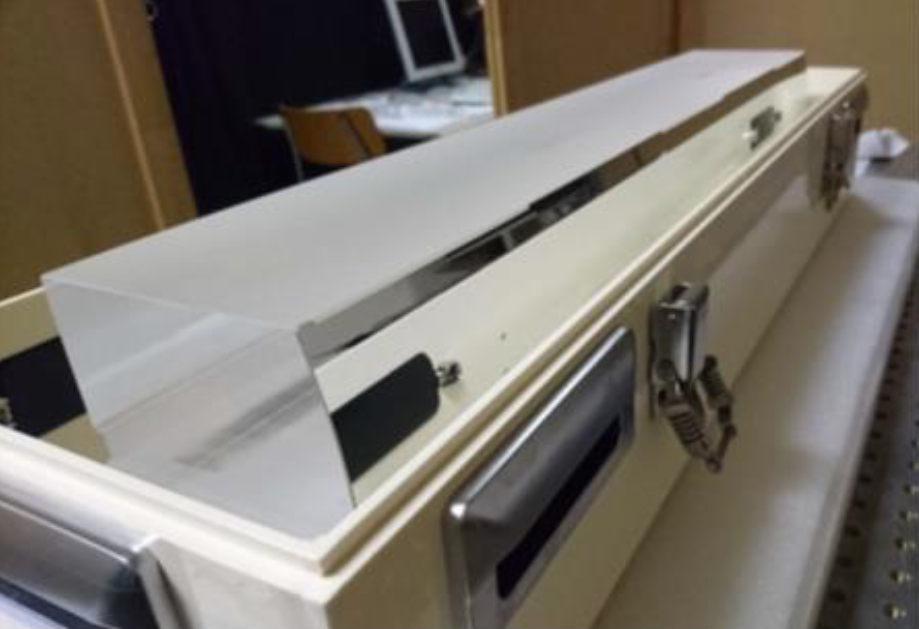
\includegraphics[width = 0.7\textwidth]{Figs/FocusingBlock_lab.png}
      \end{figure}
    \end{column}
    \begin{column}{0.35\textwidth}
      \begin{figure}
        \centering
        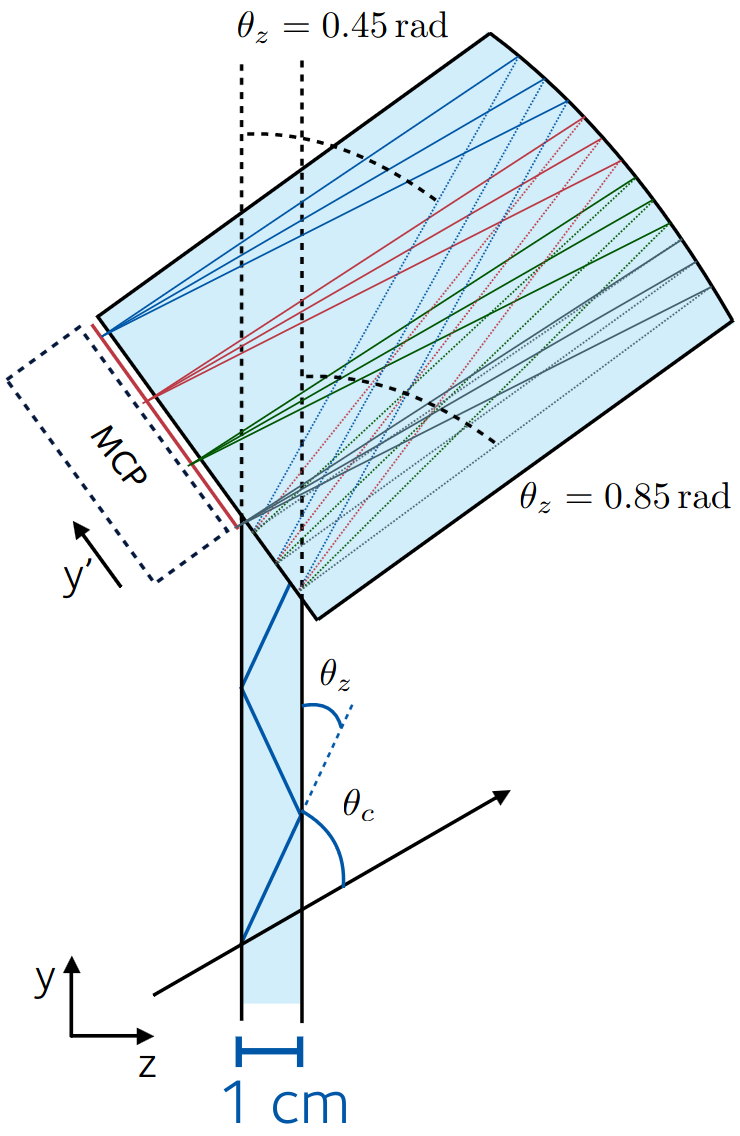
\includegraphics[width = 1.0\textwidth]{Figs/TORCH_SideView.png}
      \end{figure}
    \end{column}
  \end{columns}
\end{frame}

\section{2018 test beam analysis}
\begin{frame}{2018 test beam analysis}
  \vspace{0.0cm}
  \begin{center}
    {\large 2018 test beam analysis paper \href{https://www.sciencedirect.com/science/article/pii/S0168900223001717}{published} earlier this year}
  \end{center}
  \begin{itemize}
    \setlength\itemsep{0.3em}
    \item{$\SI{8}{\giga\eV}$ beam of pions and protons from the CERN T9 beamline}
    \item{Single-photon resolution down to $\SI{70}{\pico\second}$ achieved}
  \end{itemize}
  \begin{figure}
    \centering
    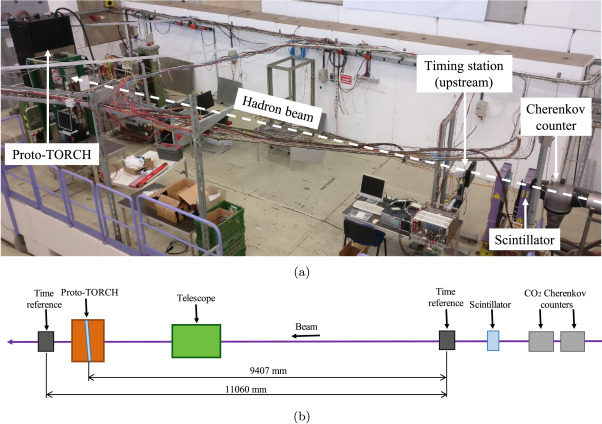
\includegraphics[width = 0.65\textwidth]{Figs/TORCH_testbeam_2018_setup.jpg}
  \end{figure}
\end{frame}

\begin{frame}{2018 test beam analysis}
  \begin{columns}
    \begin{column}{0.6\textwidth}
      \begin{itemize}
        \setlength\itemsep{1.0em}
        \item{Prototype of TORCH}
        \item{Full width, half height}
        \item{Nikon glass with polished surfaces}
      \end{itemize}
      \begin{figure}
        \centering
        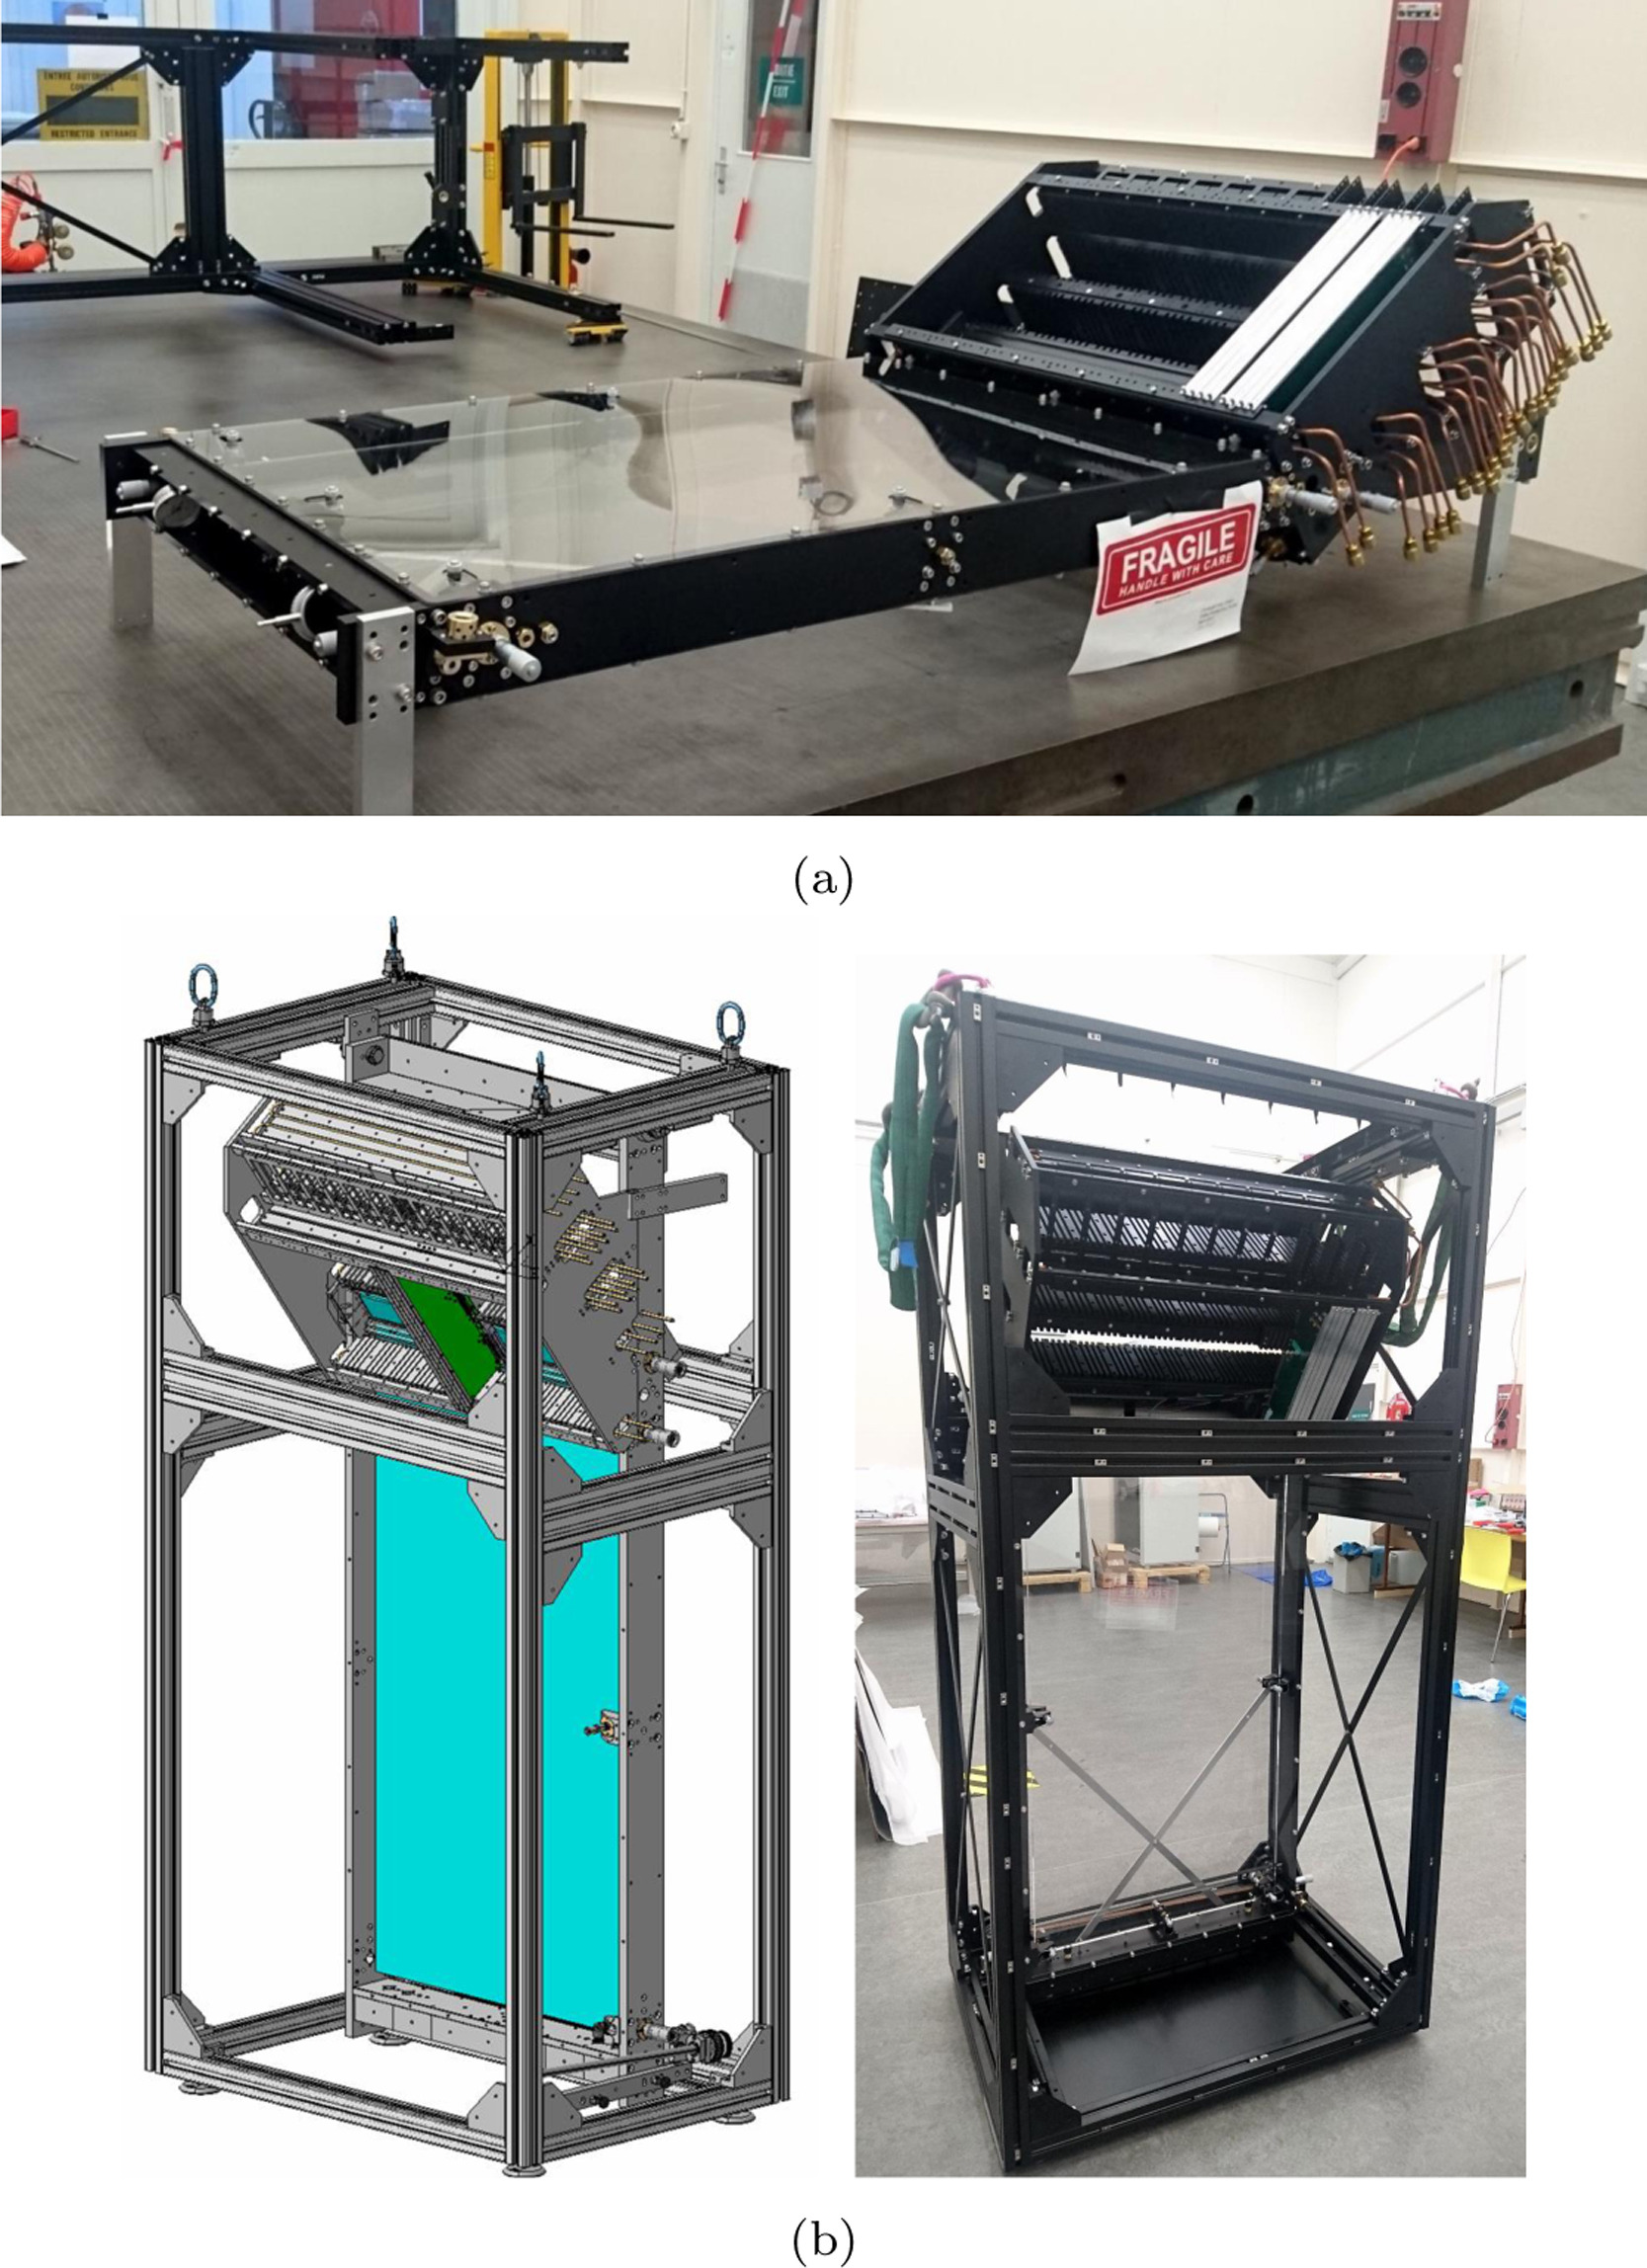
\includegraphics[width = 0.7\textwidth,trim={0 7.5cm 0 0},clip=true]{Figs/TORCH_testbeam_2018_structure.jpg}
      \end{figure}
    \end{column}
    \begin{column}{0.4\textwidth}
      \begin{figure}
        \centering
        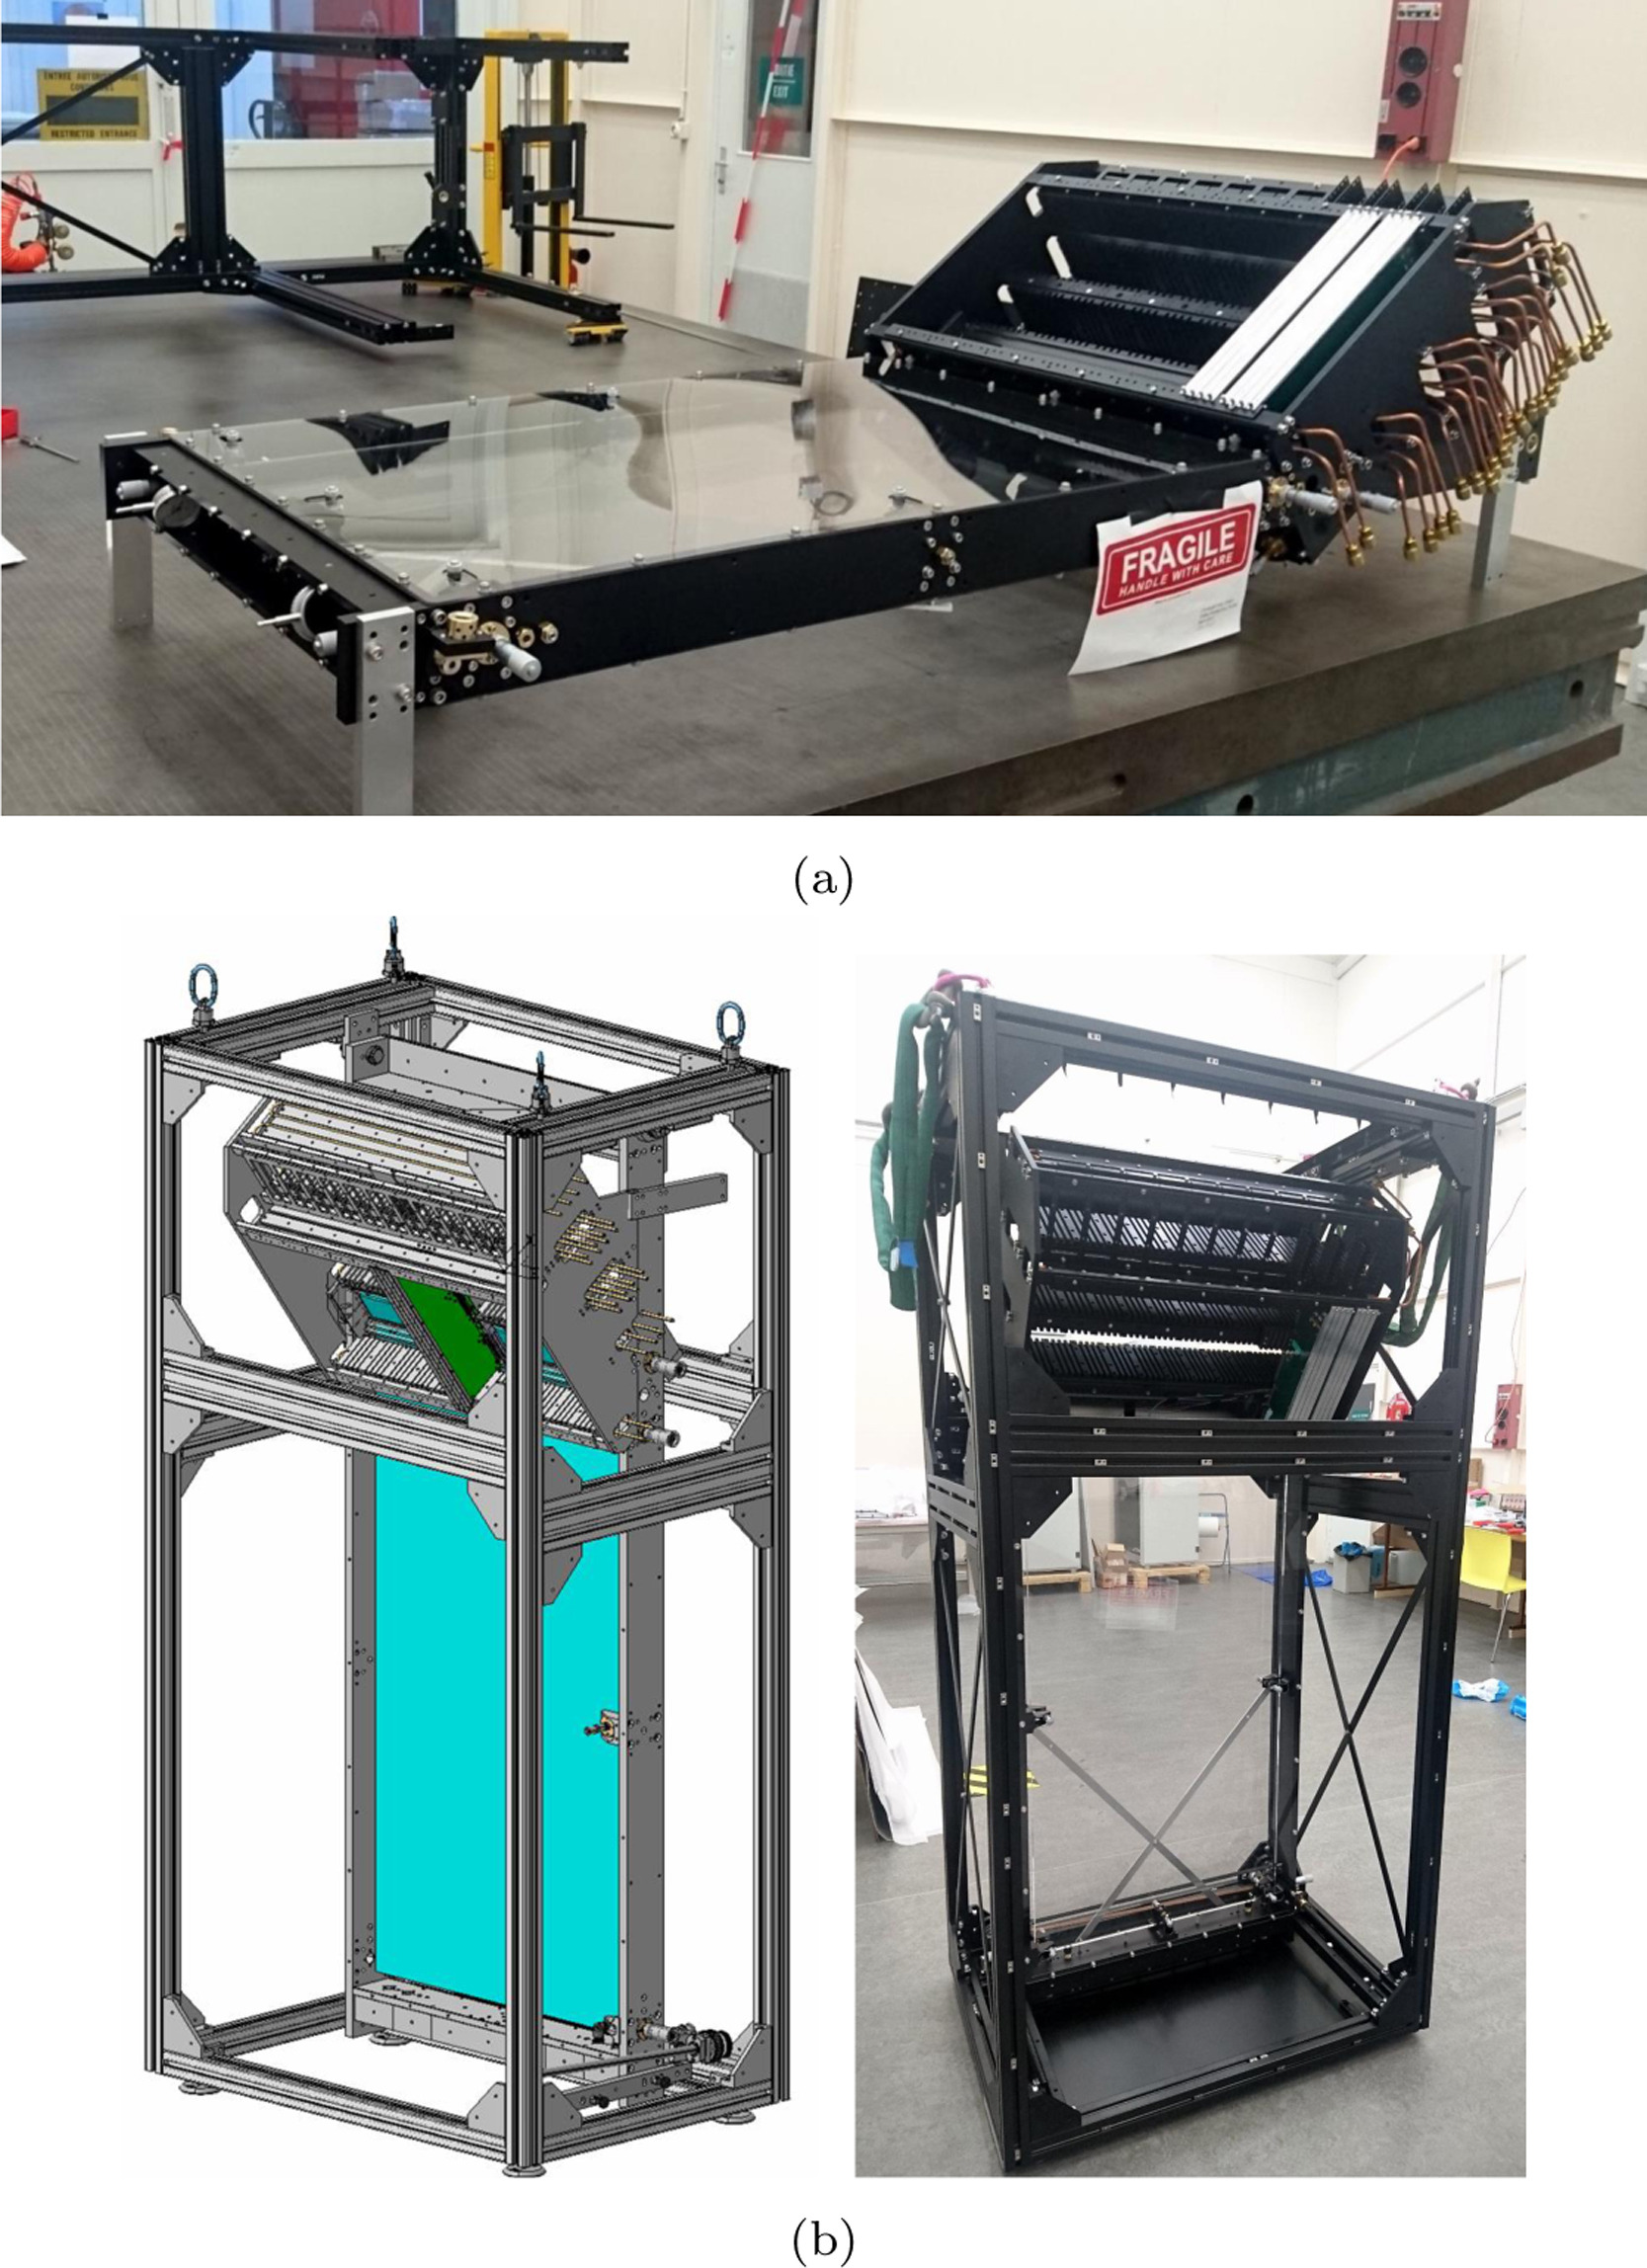
\includegraphics[width = 0.9\textwidth,trim={4.5cm 0.5cm 0 5cm},clip=true]{Figs/TORCH_testbeam_2018_structure.jpg}
      \end{figure}
    \end{column}
  \end{columns}
\end{frame}

\begin{frame}{2018 test beam analysis}
  \begin{itemize}
    \setlength\itemsep{1.0em}
    \item{Photon detector: MicroChannel Plate PhotoMultiplier Tube}
    \item{$53\times 53\si{\milli\meter\squared}$ active area}
    \item{$8$ columns, each with $64$ pixels}
    \item{Effectively $128$ pixels with charge sharing}
  \end{itemize}
  \begin{figure}
    \centering
    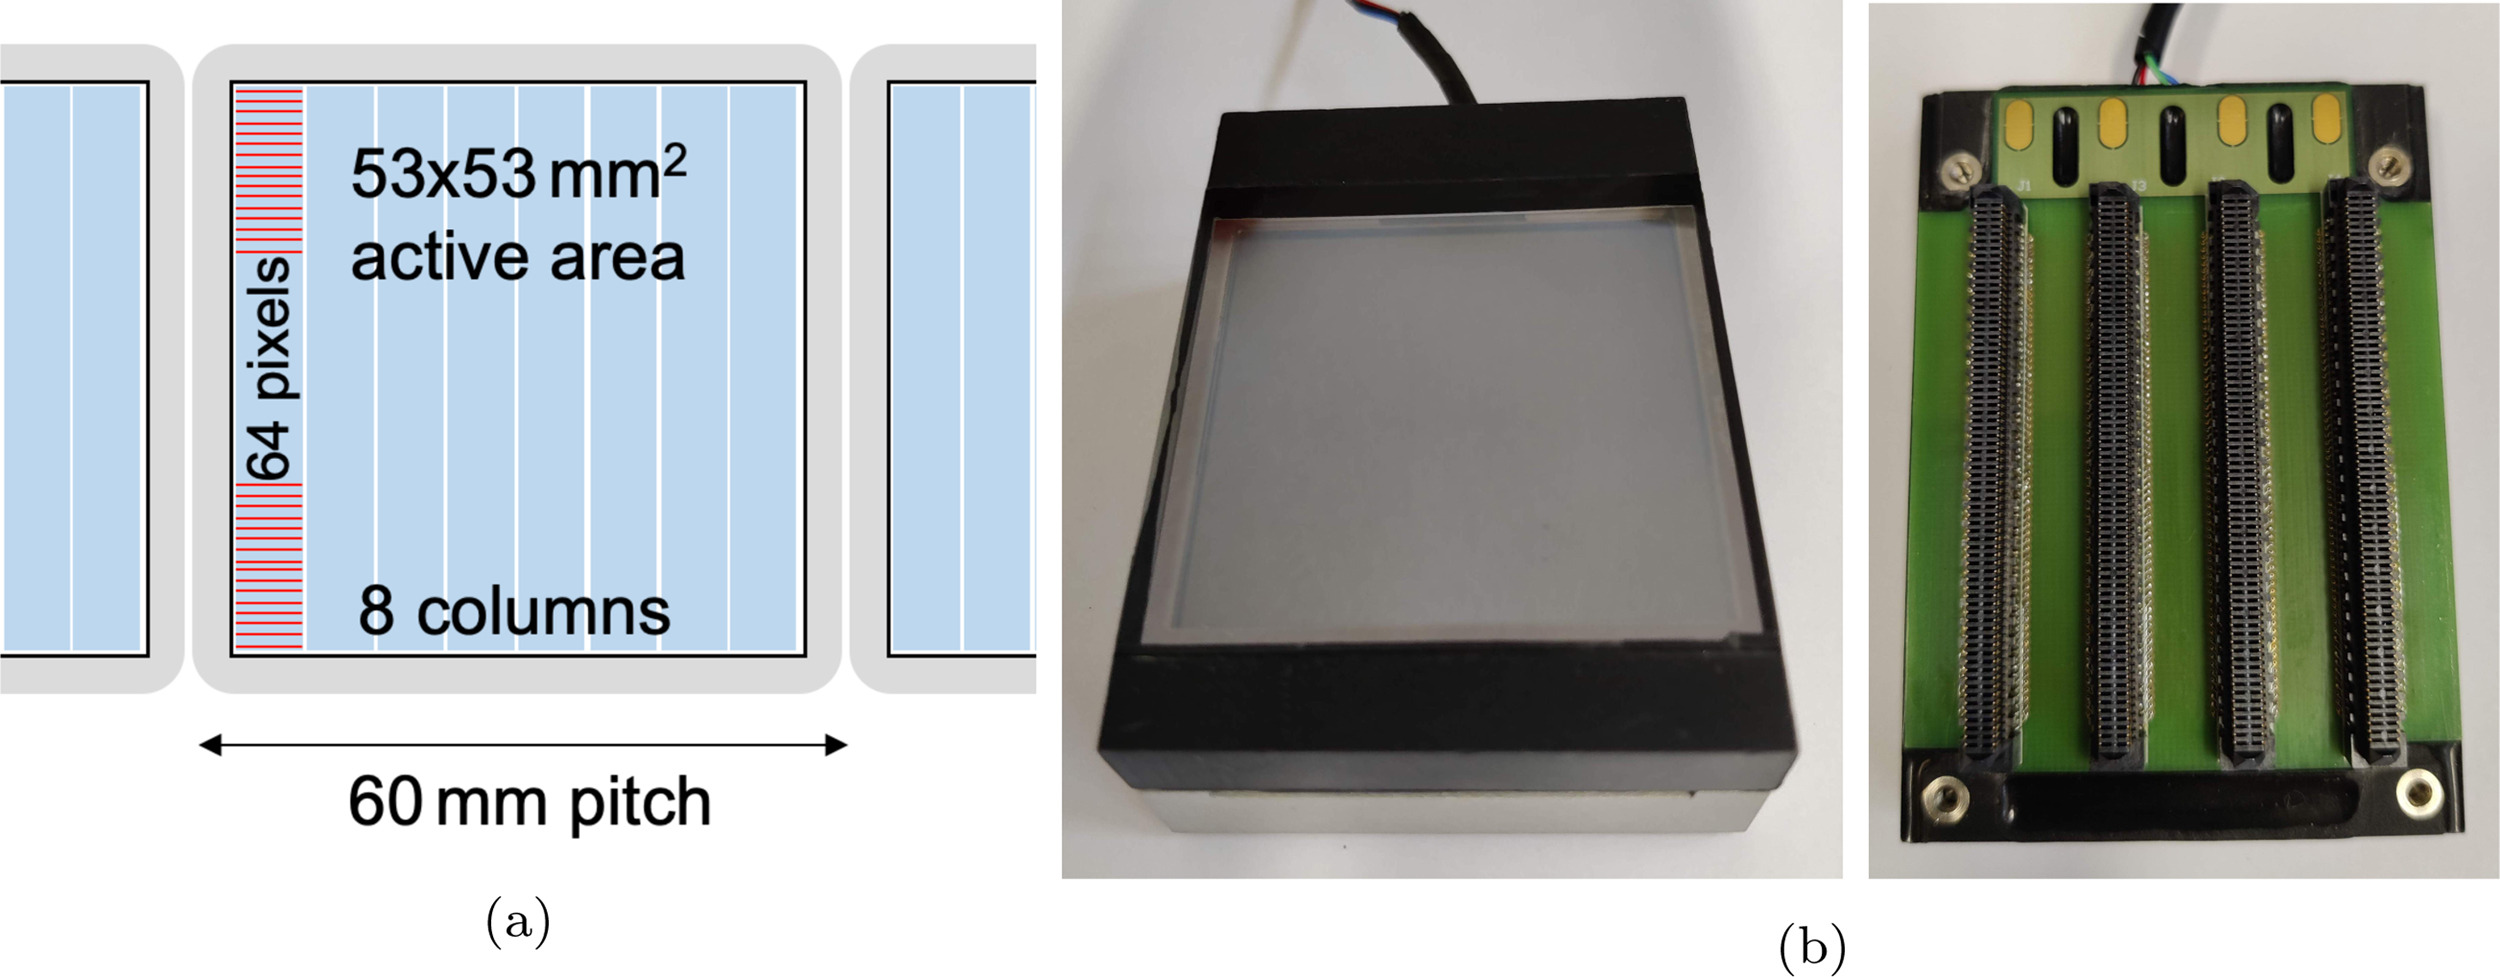
\includegraphics[width = 1.0\textwidth,trim={0 0.5cm 0 0},clip=true]{Figs/TORCH_testbeam_2018_MCPPMT.jpg}
  \end{figure}
\end{frame}

\begin{frame}{2018 test beam analysis}
  \begin{itemize}
    \setlength\itemsep{1.0em}
    \item{Photon detector: MicroChannel Plate PhotoMultiplier Tube}
    \item{$53\times 53\si{\milli\meter\squared}$ active area}
    \item{$8$ columns, each with $64$ pixels}
    \item{Effectively $128$ pixels with charge sharing}
  \end{itemize}
  \vspace{-0.35cm}
  \begin{figure}
    \centering
    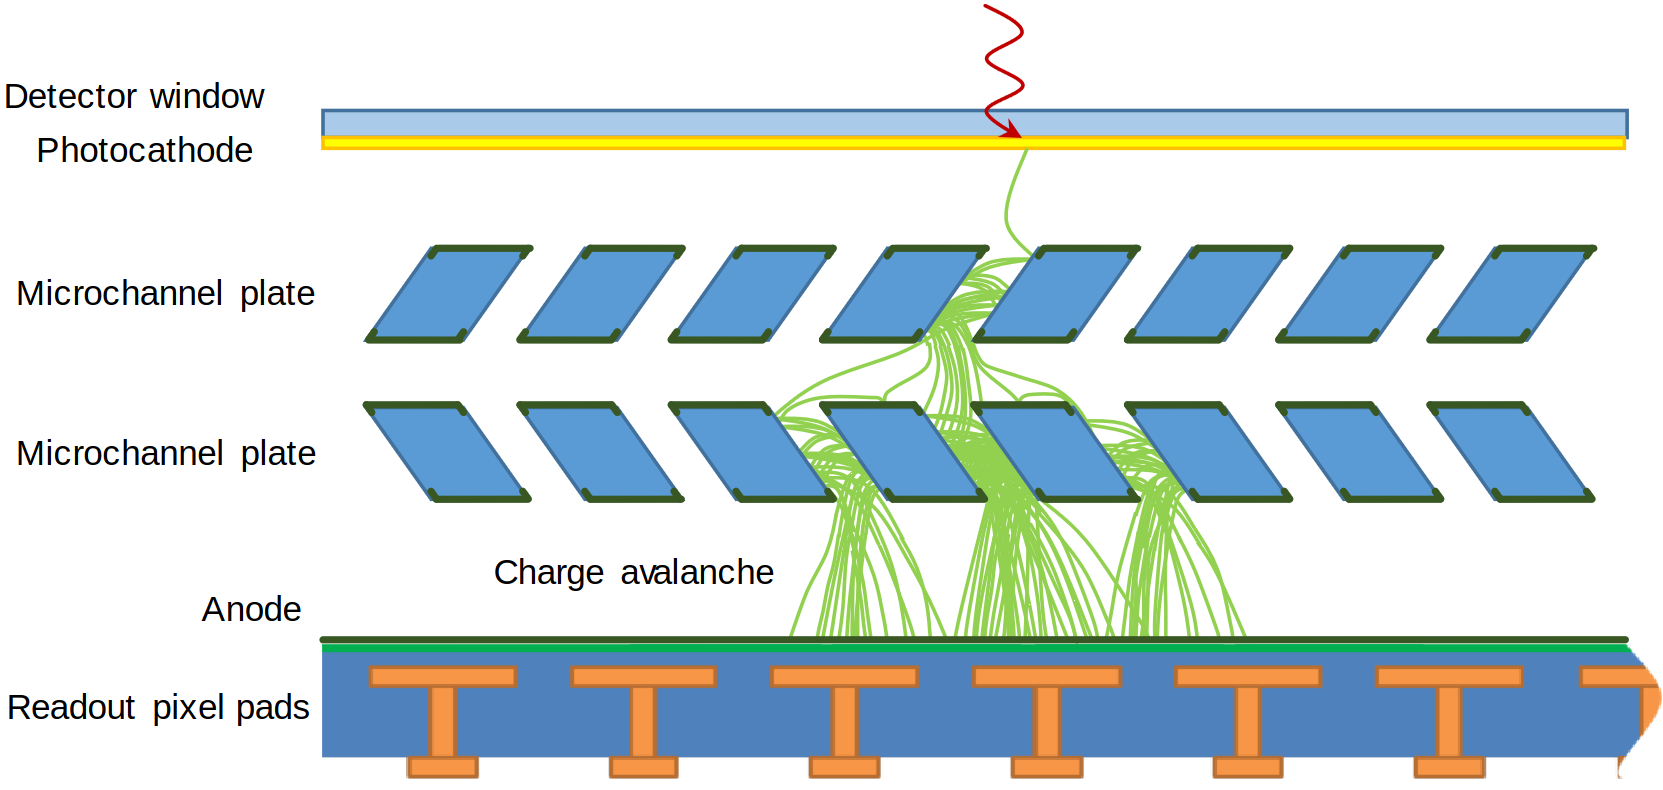
\includegraphics[width = 0.8\textwidth]{Figs/MCP_PMT_illustration.png}
  \end{figure}
\end{frame}

\begin{frame}{2018 test beam analysis}
  \begin{itemize}
    \setlength\itemsep{1.0em}
    \item{NINO: Amplifier and discriminator}
    \item{High Performance Time to Digital Converter: $\SI{100}{\pico\second}$ bins}
    \item{Legacy electronics that will be replaced, more on this later!}
  \end{itemize}
  \begin{figure}
    \centering
    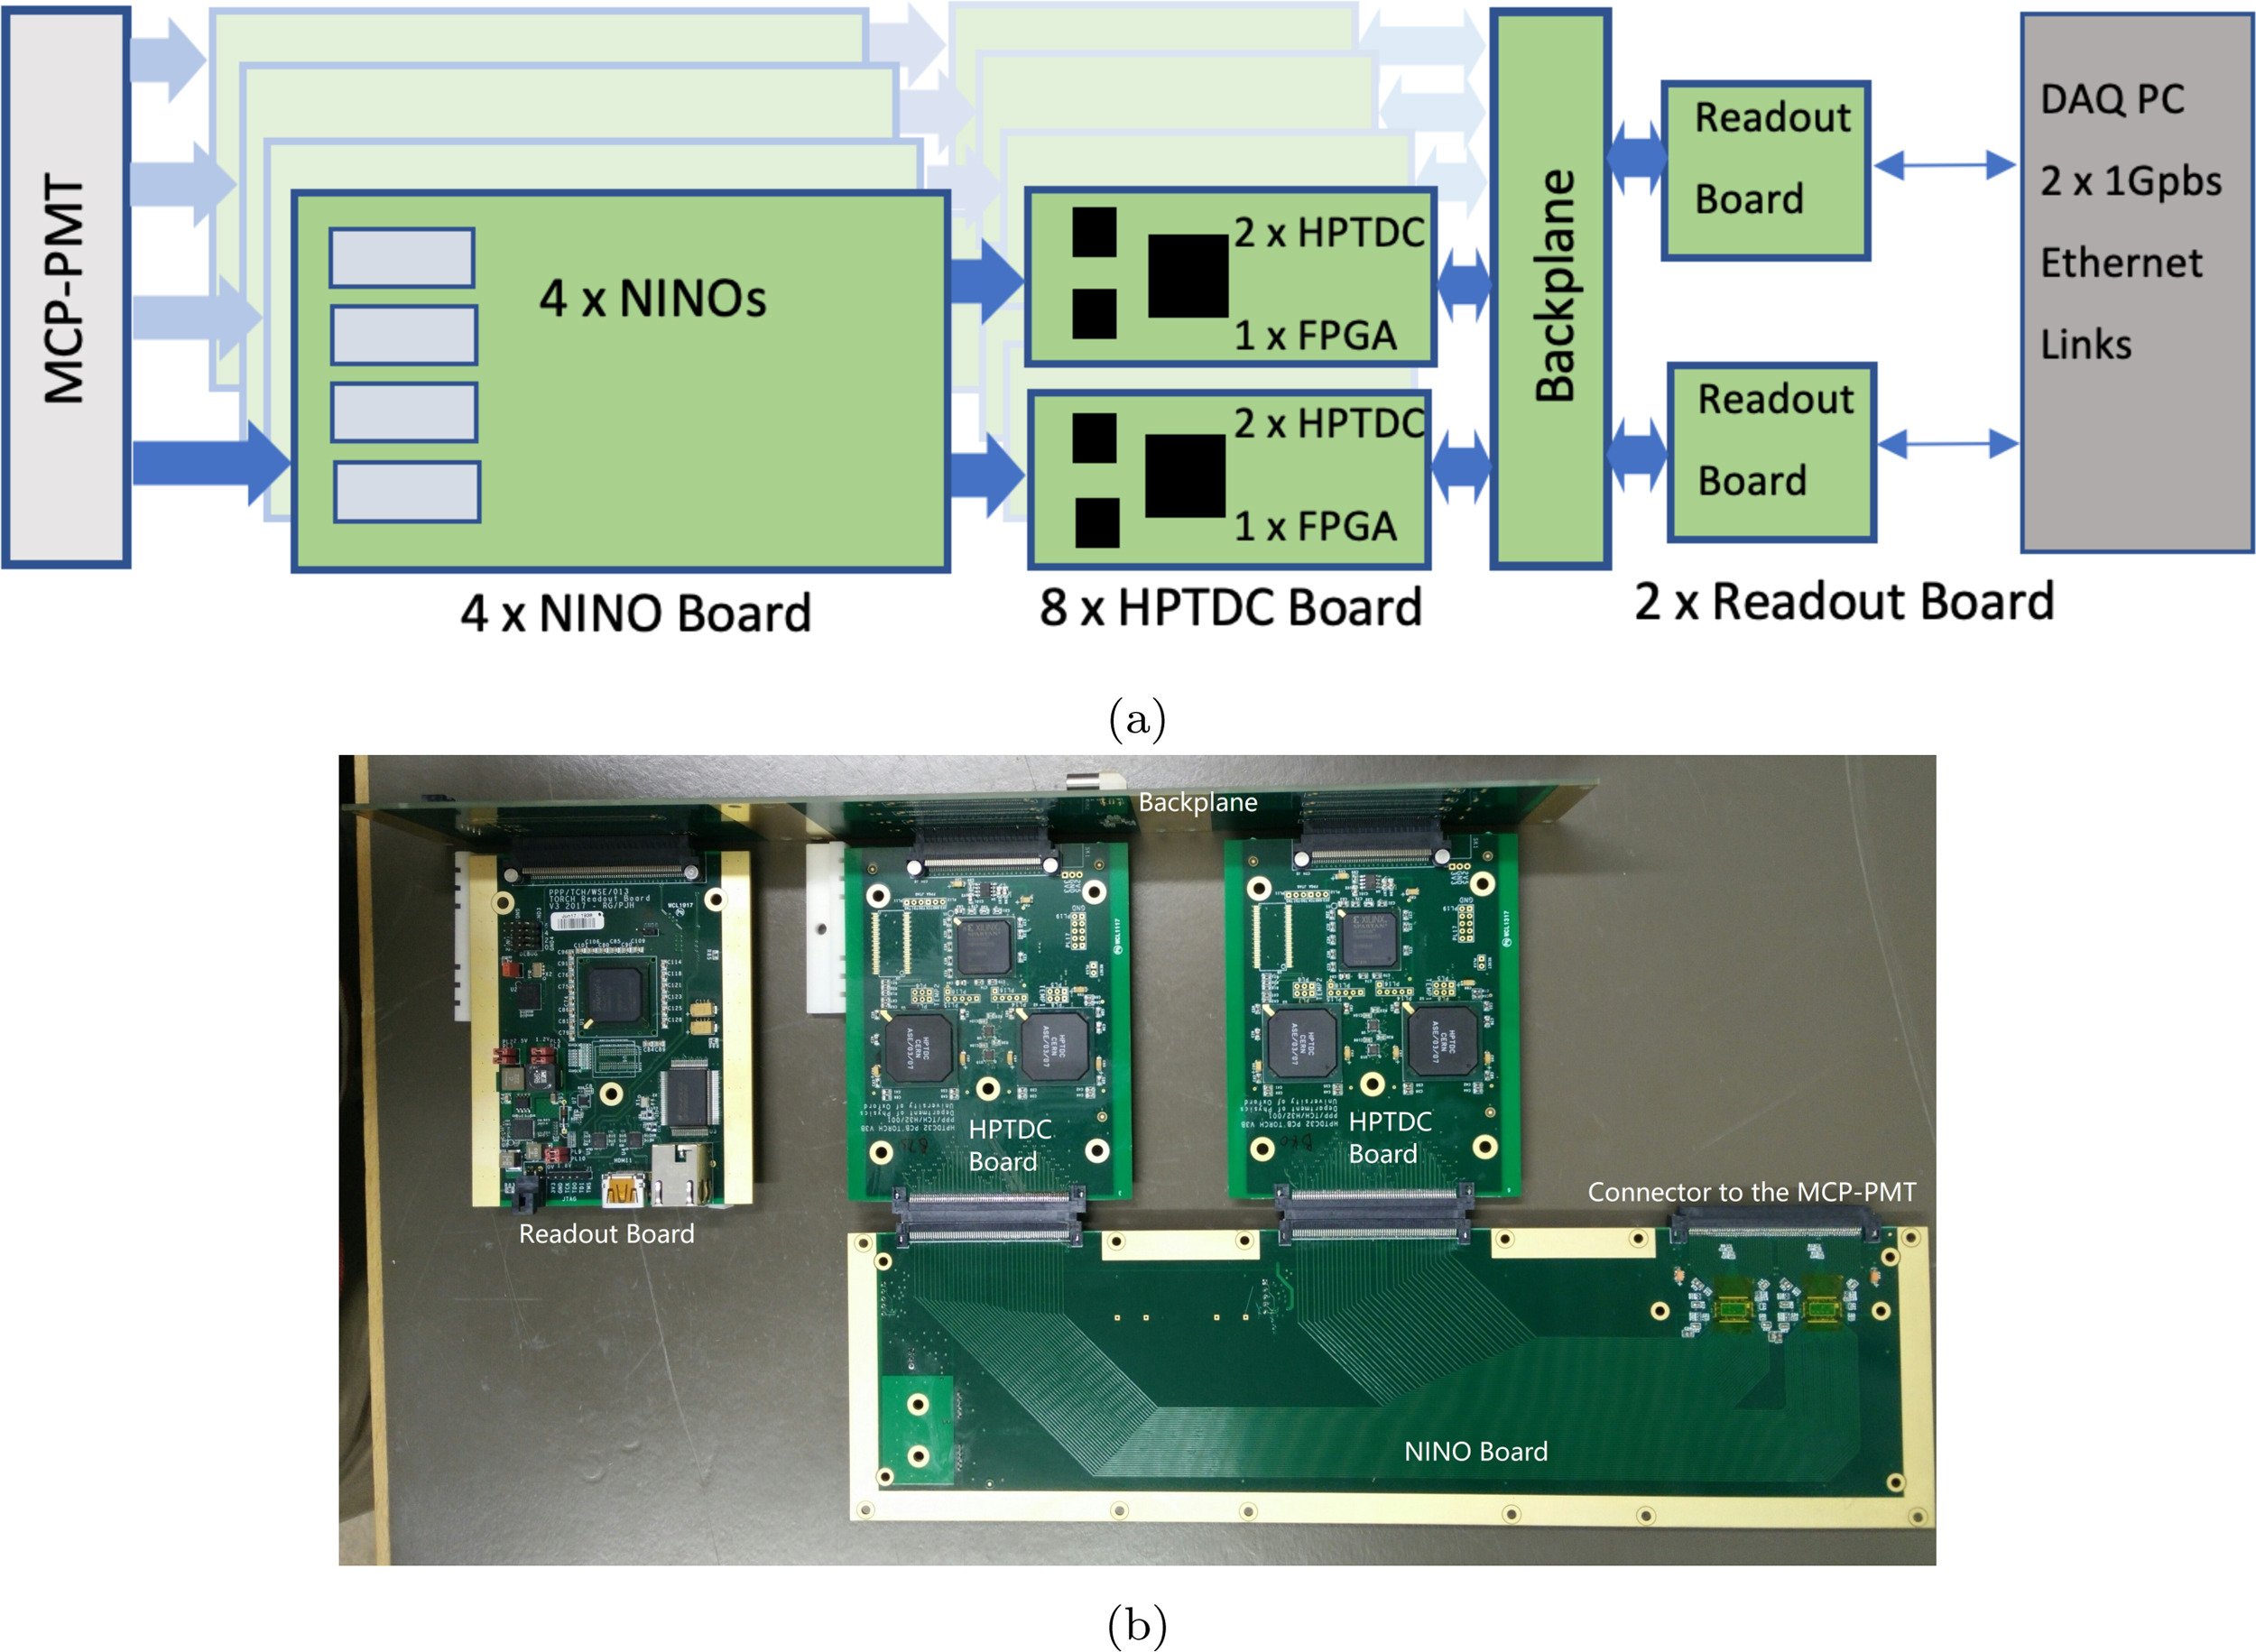
\includegraphics[width = 1.0\textwidth,trim={0 0.3cm 0 4.2cm},clip=true]{Figs/TORCH_testbeam_2018_electronics.jpg}
  \end{figure}
\end{frame}

\begin{frame}{2018 test beam analysis}
  \begin{itemize}
    \setlength\itemsep{1.0em}
    \item{Time resolution down to $\SI{70}{\pico\second}$}
    \item{Worse resolution for tracks entering at the bottom}
    \begin{itemize}
      \item{Uncertainty in chromatic dispersion scales with photon path length}
      \item{Improvements expected with further electronics calibrations}
    \end{itemize}
  \end{itemize}
  \begin{figure}
    \centering
    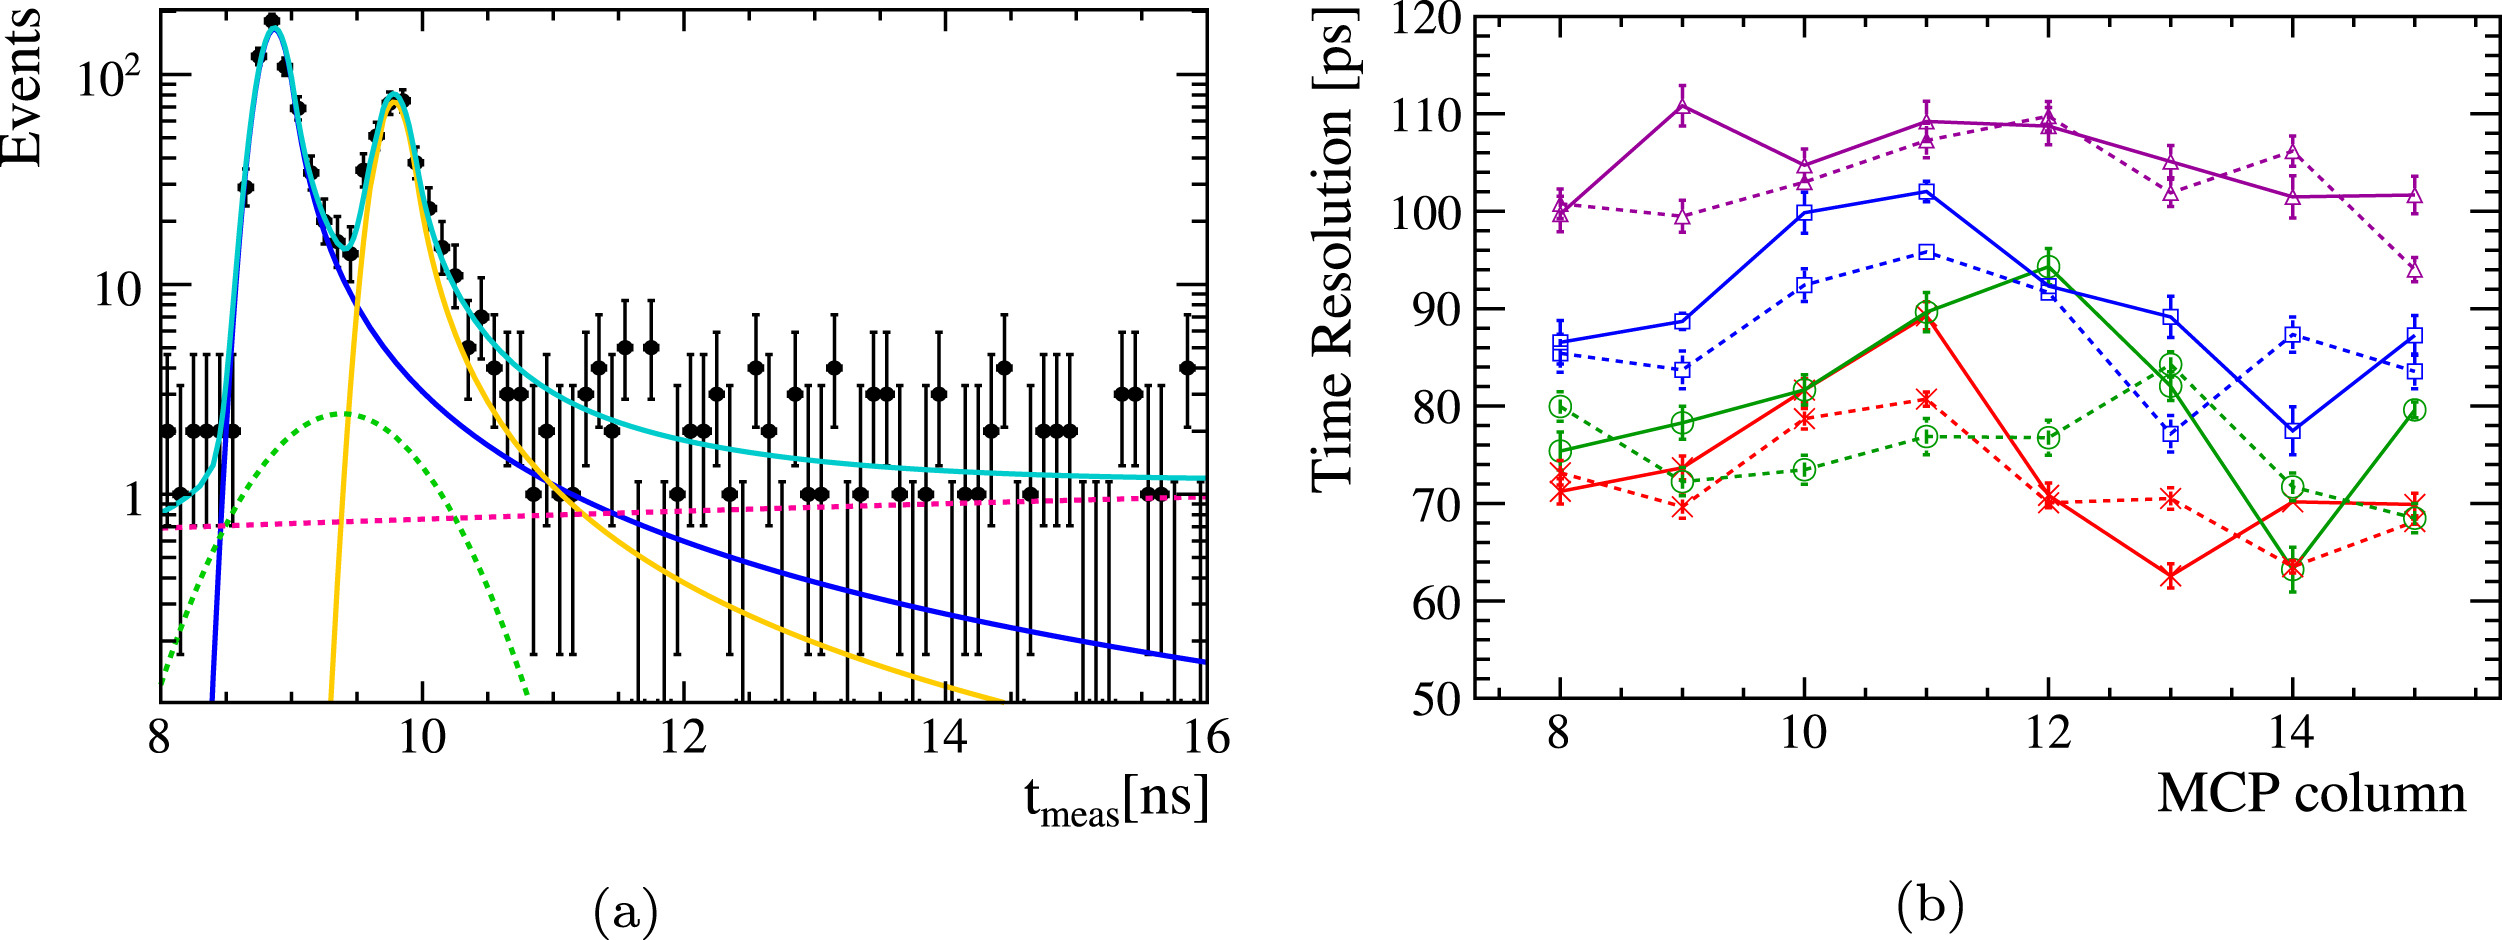
\includegraphics[width = 1.0\textwidth]{Figs/TORCH_testbeam_2018_TimeResolution.jpg}
  \end{figure}
\end{frame}

\section{2022 test beam analysis}
\begin{frame}{2022 test beam analysis}
  \vspace{0.0cm}
  \begin{center}
    {\large Back to T9, with several new goals:}
  \end{center}
  \begin{enumerate}
    \setlength\itemsep{1.0em}
    \item{Additional, fully instrumented, MCP-PMT tubes (7 in total)}
    \item{Wide range of beam momenta ($3$, $5$, $8$, $\SI{10}{\giga\eV}$ and higher)}
    \item{First demonstration of PID separation in TORCH}
  \end{enumerate}
  \begin{figure}
    \centering
    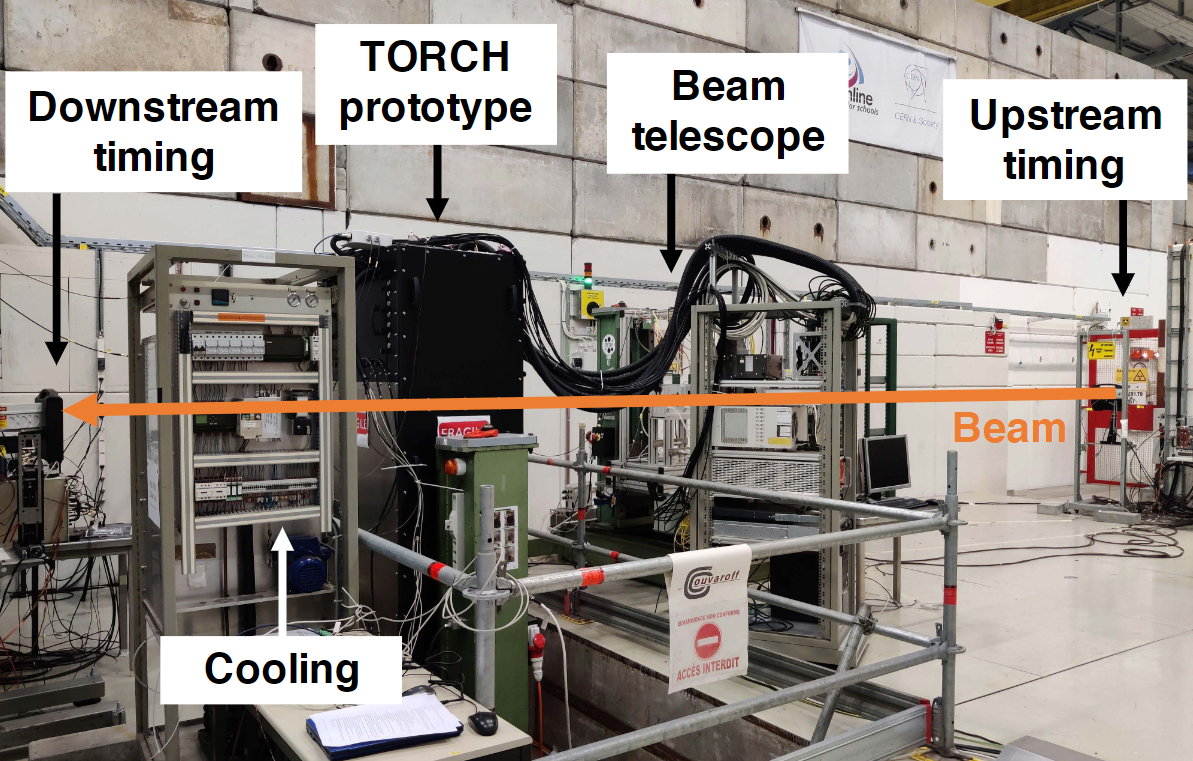
\includegraphics[width = 0.6\textwidth]{Figs/TORCH_overview.png}
  \end{figure}
\end{frame}

\begin{frame}{2022 test beam analysis}
  \vspace{0.0cm}
  \begin{center}
    {\large Global hit map looks very encouraging!}
  \end{center}
  \begin{enumerate}
    \setlength\itemsep{1.0em}
    \item{Hit pattern seen across 6 MCP-PMT tubes}
    \item{Minimal degradation of original MCP A and B}
    \item{Proper time reference channel present in (almost) all columns}
  \end{enumerate}
  \begin{figure}
    \centering
    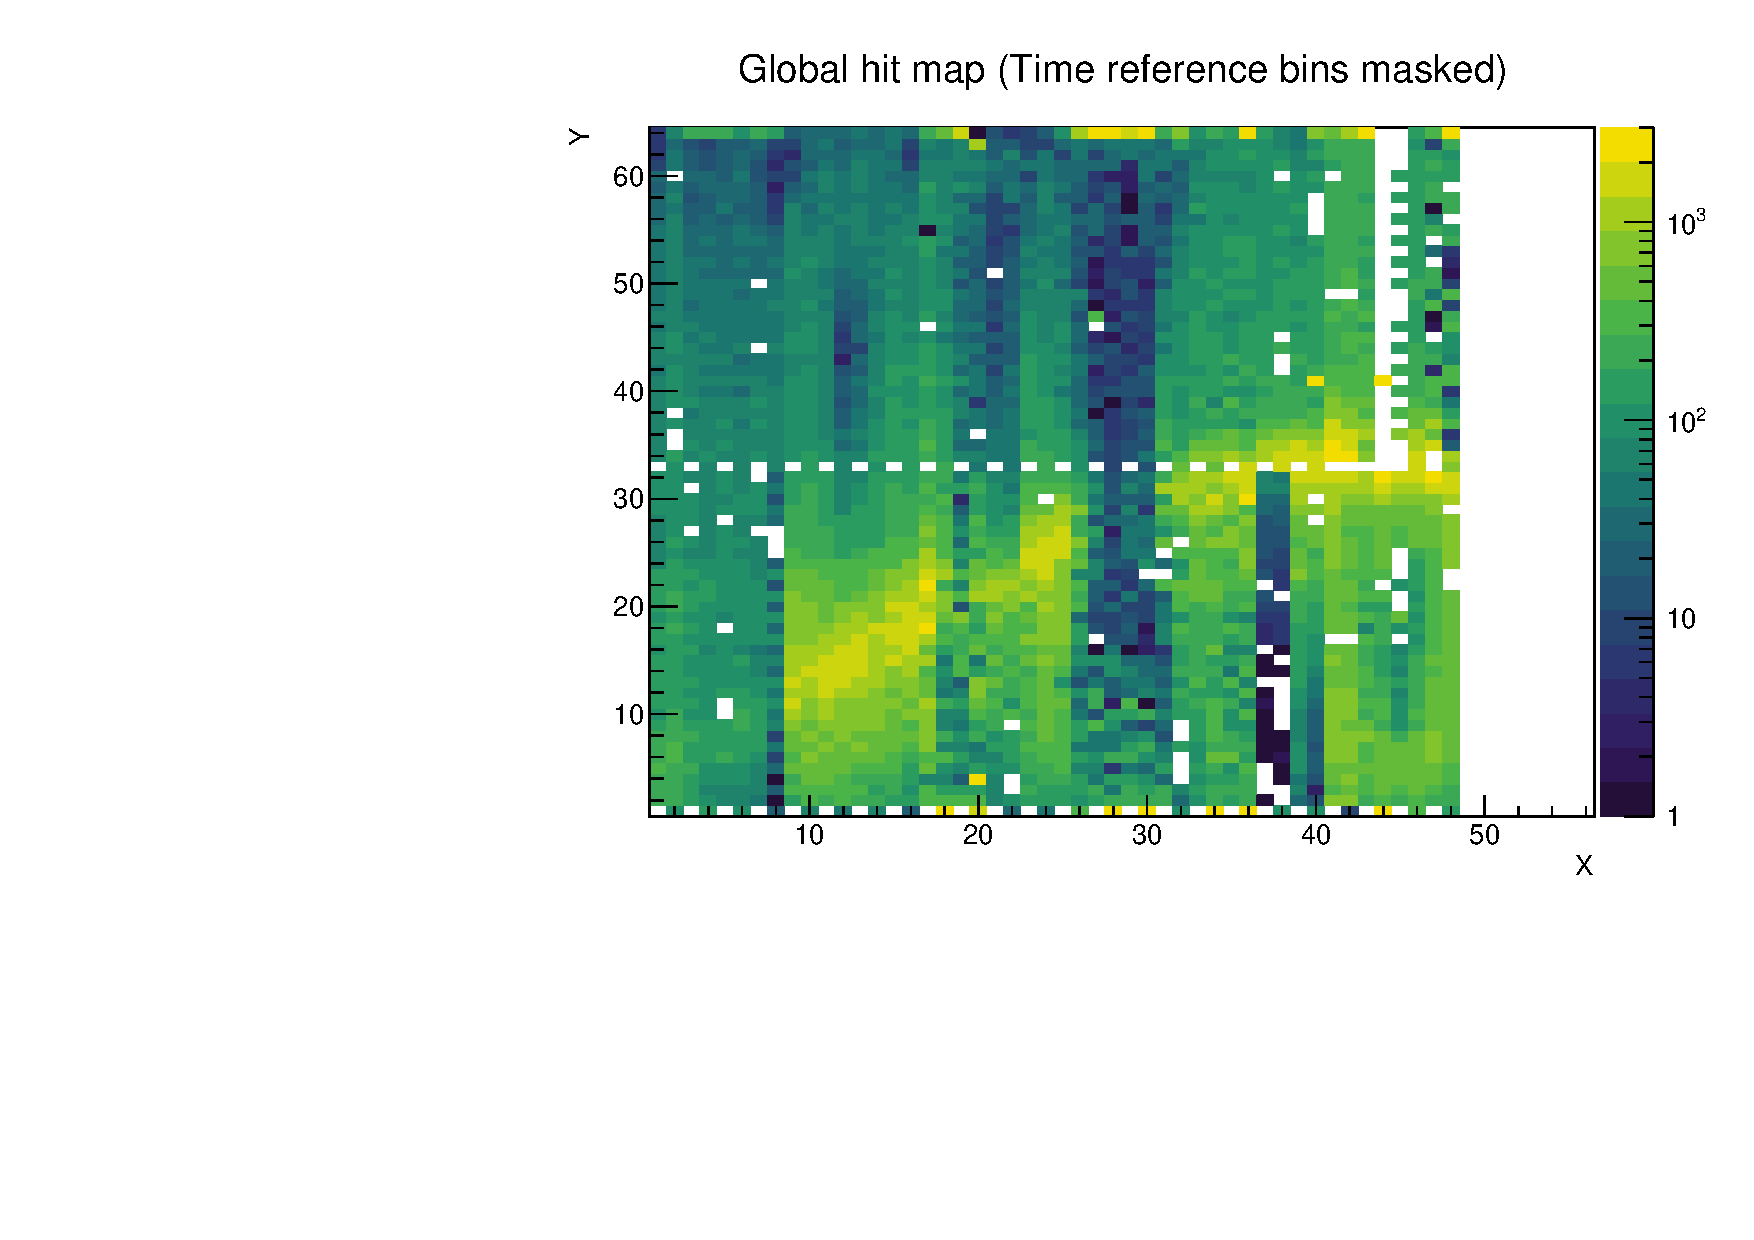
\includegraphics[width = 0.6\textwidth]{Figs/GlobalHitMap_Run480.pdf}
  \end{figure}
\end{frame}

\begin{frame}{2022 test beam analysis}
  \vspace{0.0cm}
  \begin{center}
    {\large Additional MCP tubes work well, but focus on MCP A and B for now}
  \end{center}
  \vspace{0.1cm}
  \begin{enumerate}
    \setlength\itemsep{1.0em}
    \item{Electronics of new MCPs need to be understood better}
    \begin{itemize}
      \item{Improve stability and reliability}
      \item{NINO thresholds need to be optimised}
    \end{itemize}
    \item{Some non-uniformity in QE and gain seen in MCP C, D and F}
  \end{enumerate}
  \begin{figure}
    \centering
    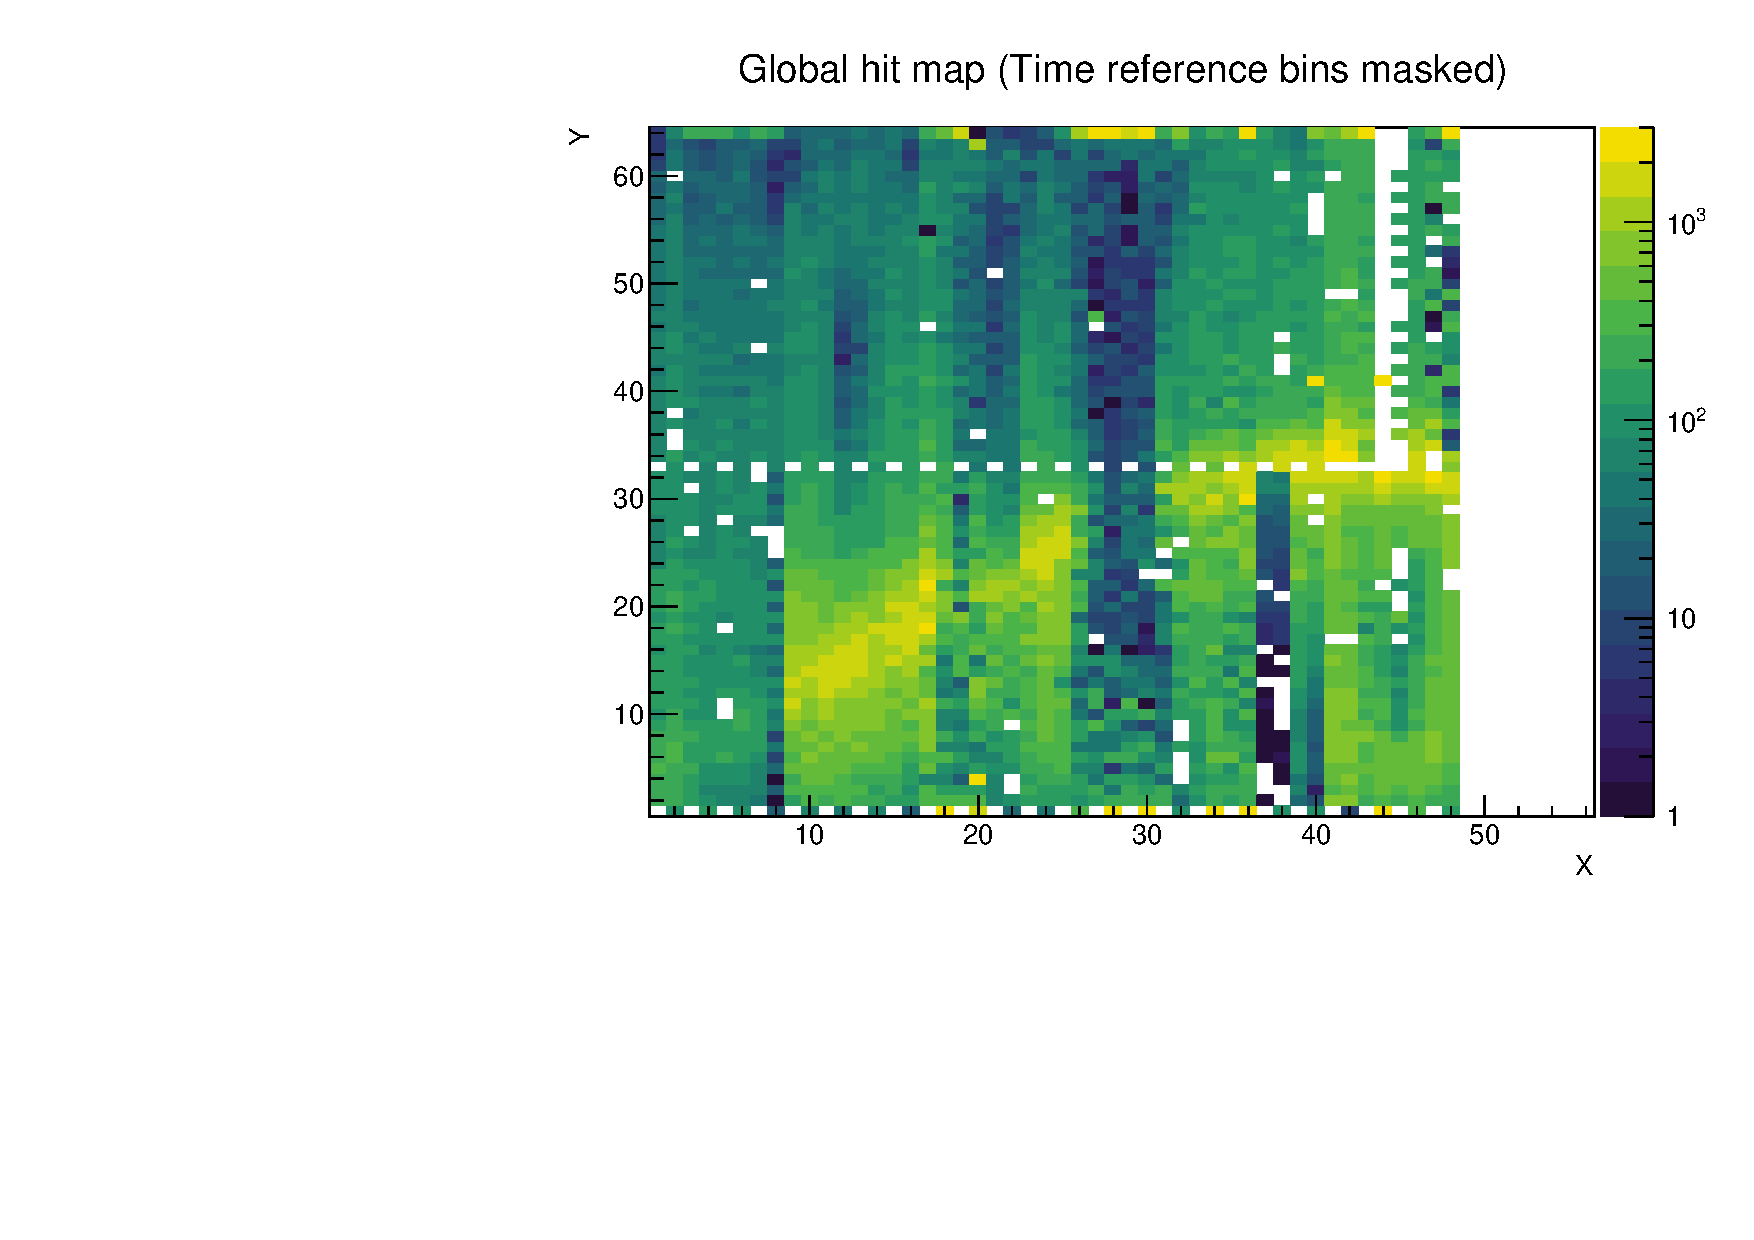
\includegraphics[width = 0.6\textwidth]{Figs/GlobalHitMap_Run480.pdf}
  \end{figure}
\end{frame}

\begin{frame}{2022 test beam analysis}
  \begin{columns}
    \begin{column}{0.7\textwidth}
      \begin{itemize}
        \setlength\itemsep{1.0em}
        \item{Study positions 1, 8, 9, 10, 11, 12}
        \item{Below: Comparison of position 1 between 2018 and 2022 data $\implies$ Perfect agreement!}
      \end{itemize}
      \vspace{-0.3cm}
      \begin{figure}
        \centering
        \caption*{2018\qquad\qquad\qquad\qquad\qquad\qquad 2022}
        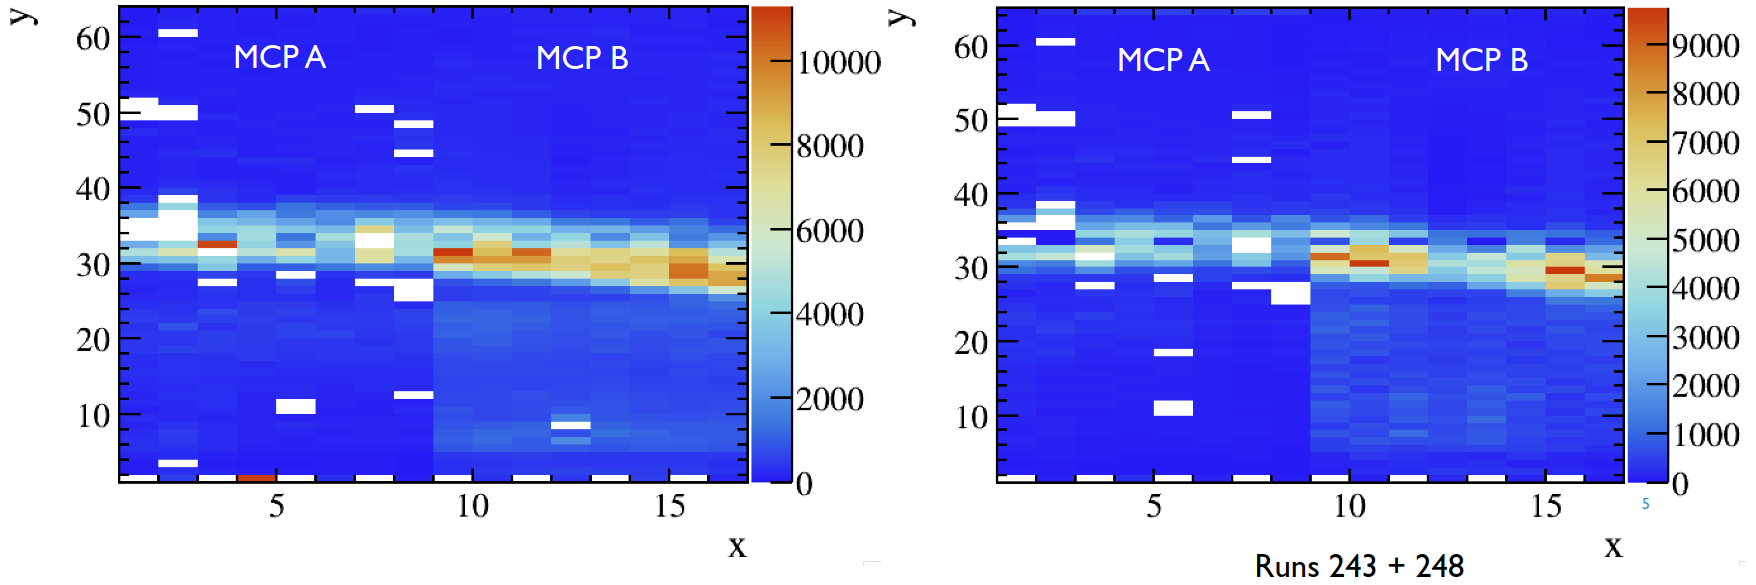
\includegraphics[width = 1.0\textwidth]{Figs/TORCH_testbeam_2018_2022_comparison.png}
      \end{figure}
      \begin{itemize}
        \item{This talk: Preliminary results from position 8}
        \begin{itemize}
          \item{Never studied before!}
        \end{itemize}
      \end{itemize}
    \end{column}
    \begin{column}{0.3\textwidth}
      \begin{figure}
        \centering
        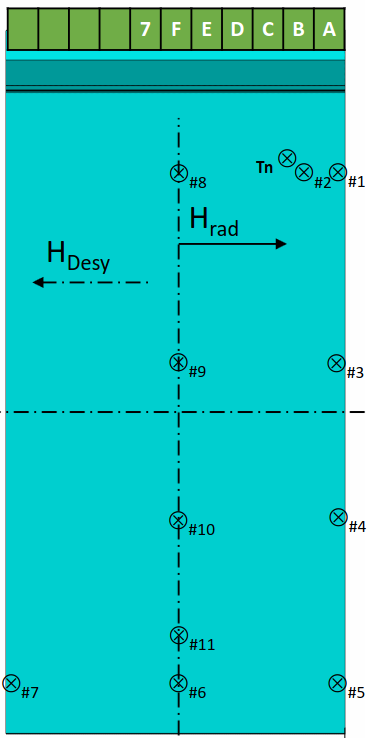
\includegraphics[width = 0.9\textwidth]{Figs/BeamPositions.png}
      \end{figure}
    \end{column}
  \end{columns}
\end{frame}

\begin{frame}{2022 test beam analysis}
  \vspace{0.0cm}
  \begin{center}
    {\large Check time of flight between time references}\\
    {\normalsize Expected time difference at $\SI{10}{\giga\eV}$: $\SI{0.15}{\nano\second}$}
  \end{center}
  \begin{figure}
    \centering
    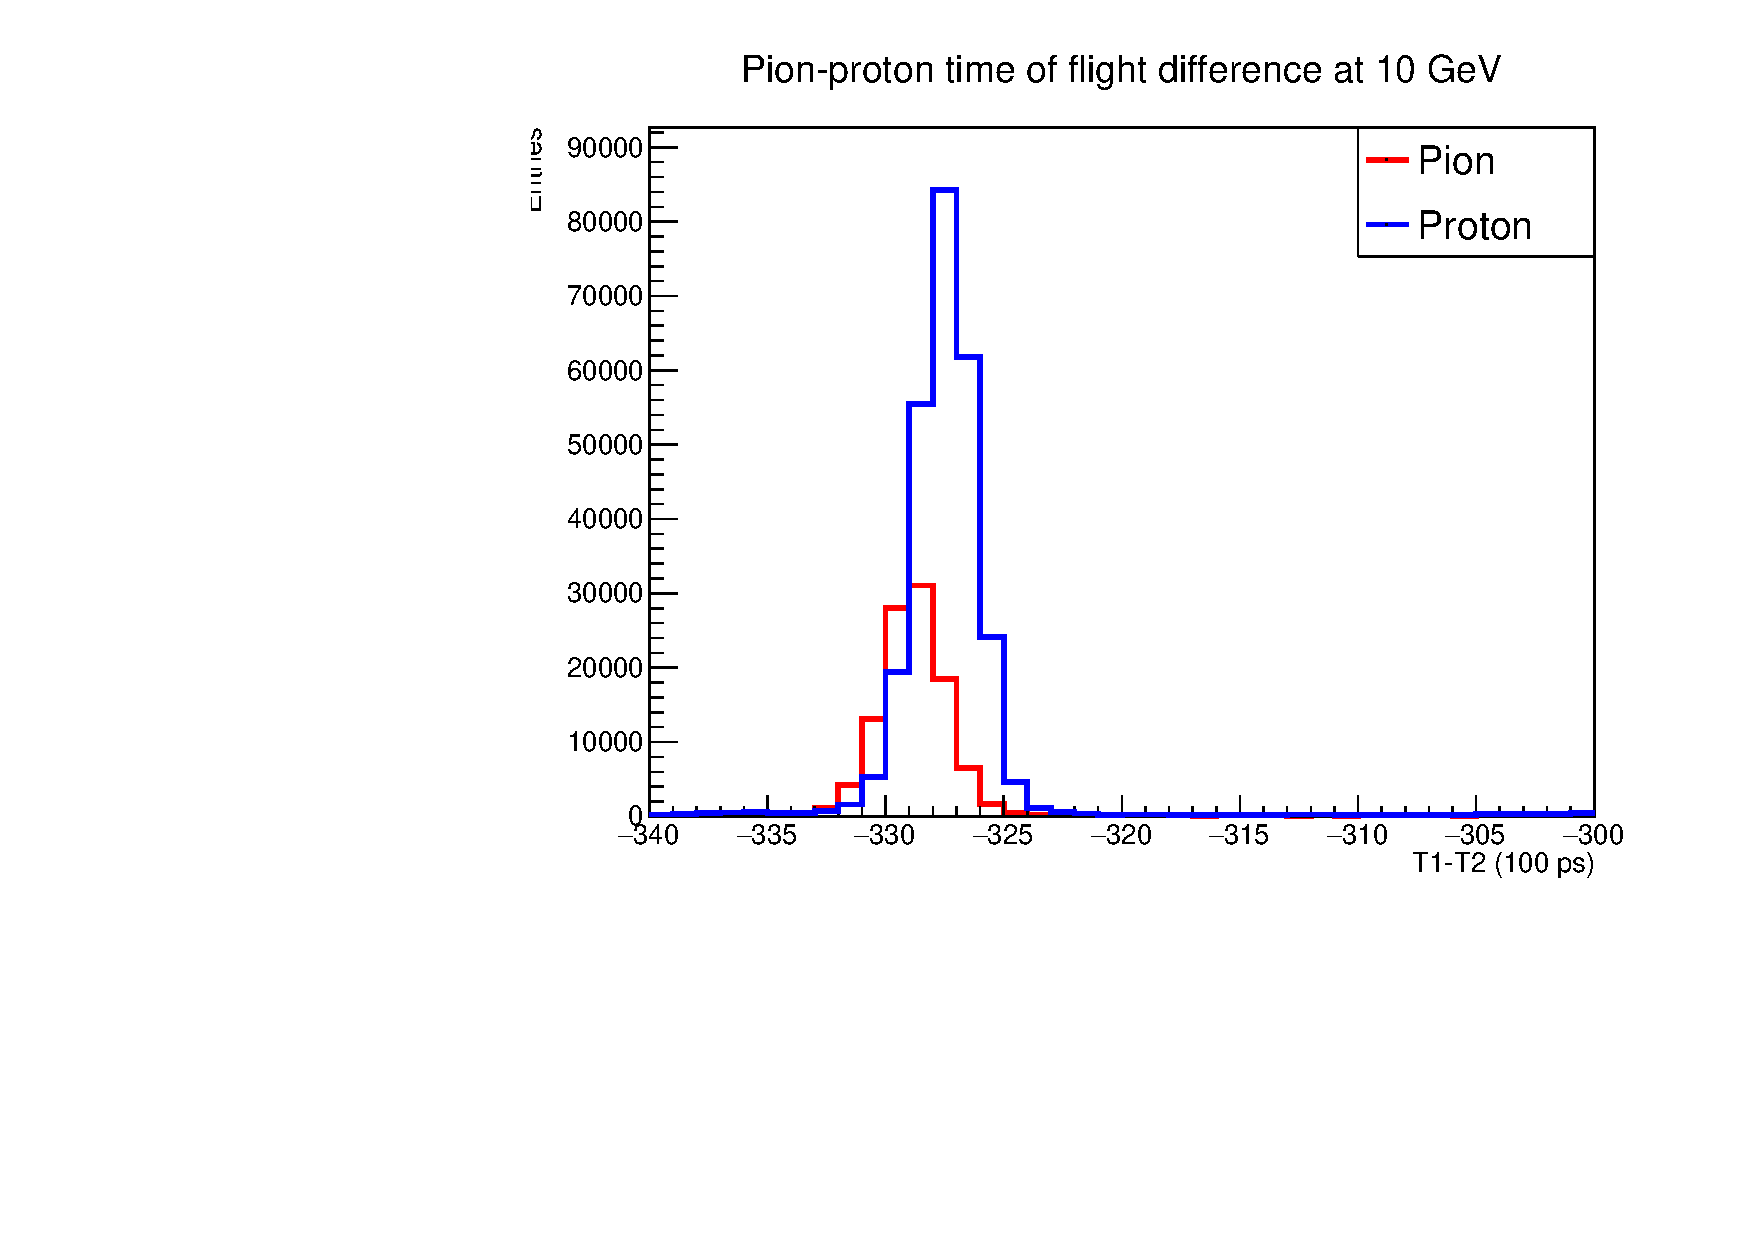
\includegraphics[width = 0.7\textwidth]{Figs/PionProton_TimeDiff_10GeV.pdf}
  \end{figure}
\end{frame}

\begin{frame}{2022 test beam analysis}
  \vspace{0.0cm}
  \begin{center}
    {\large Check time of flight between time references}\\
    {\normalsize Expected time difference at $\SI{8}{\giga\eV}$: $\SI{0.23}{\nano\second}$}
  \end{center}
  \begin{figure}
    \centering
    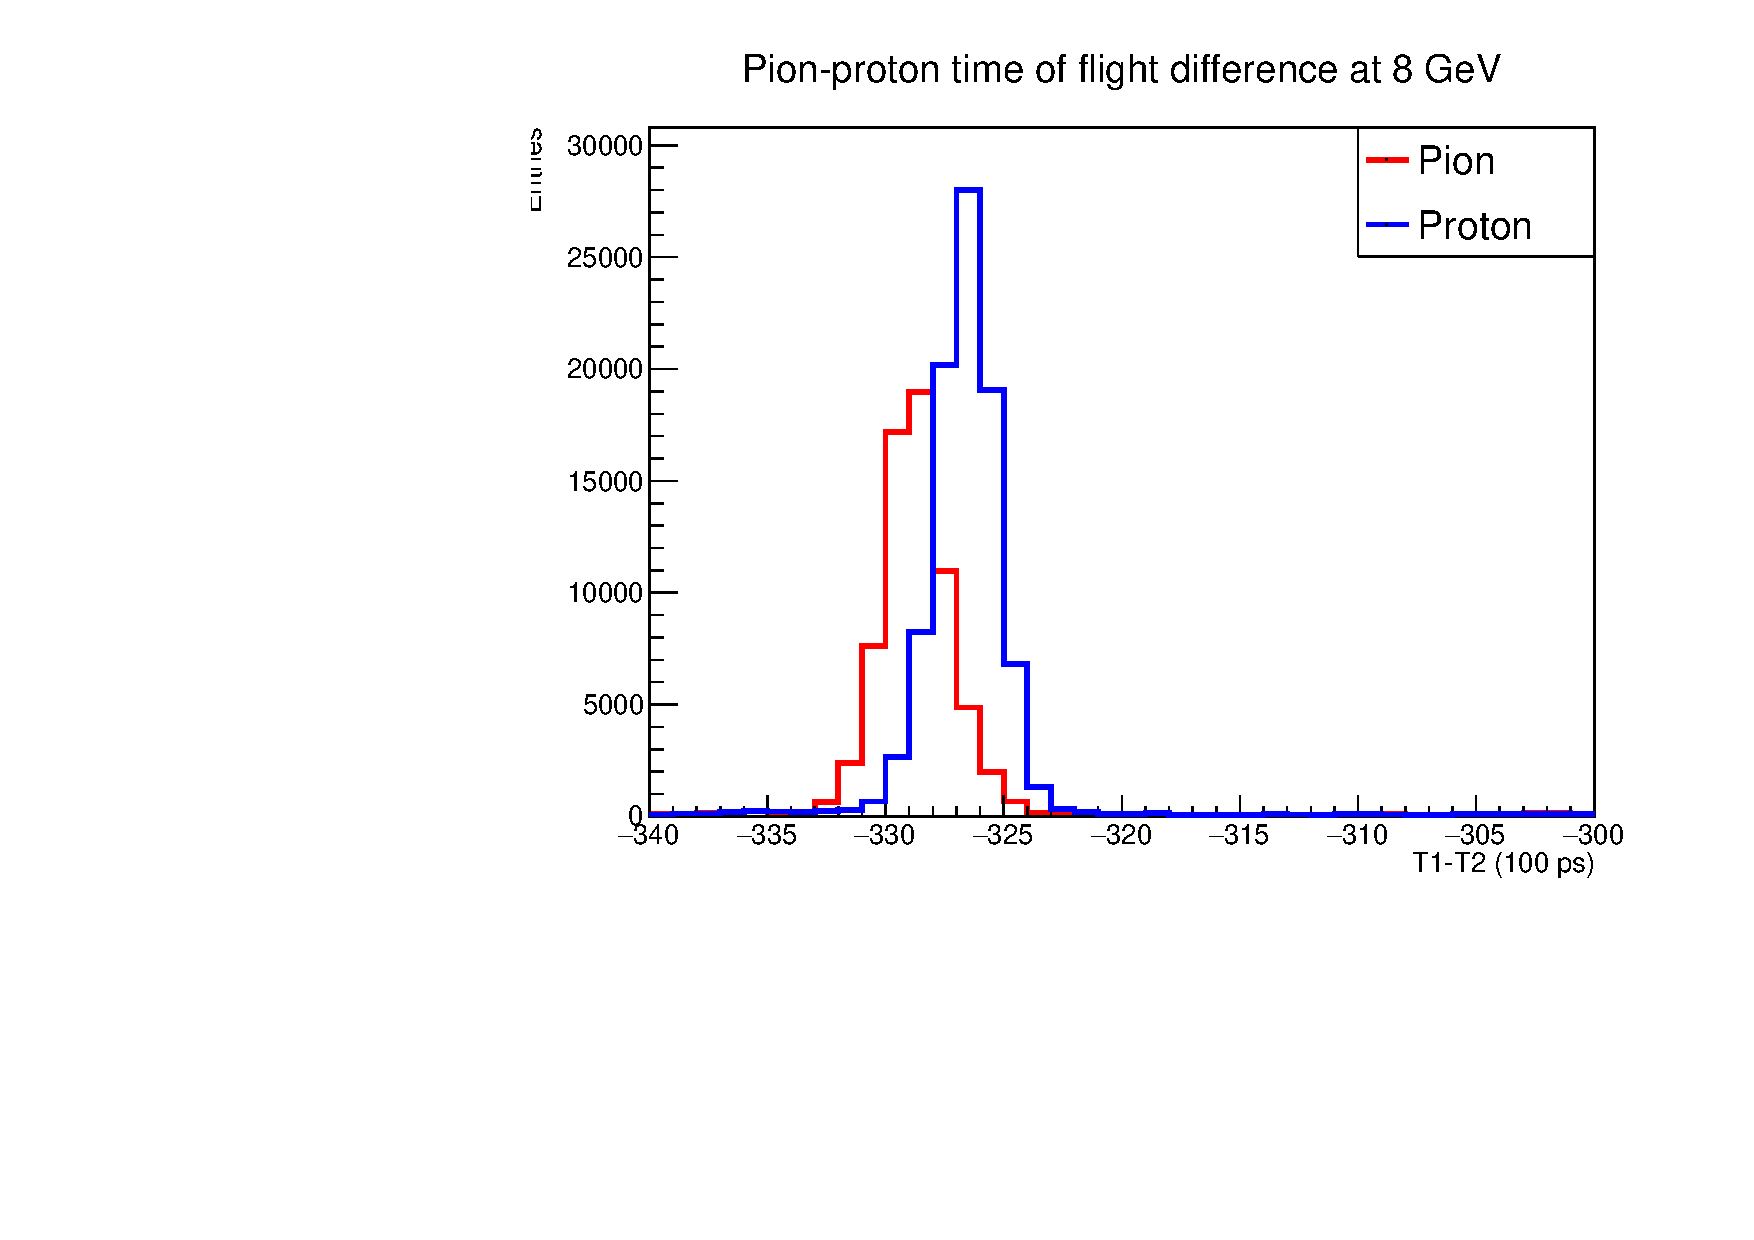
\includegraphics[width = 0.7\textwidth]{Figs/PionProton_TimeDiff_8GeV.pdf}
  \end{figure}
\end{frame}

\begin{frame}{2022 test beam analysis}
  \vspace{0.0cm}
  \begin{center}
    {\large Check time of flight between time references}\\
    {\normalsize Expected time difference at $\SI{5}{\giga\eV}$: $\SI{0.59}{\nano\second}$}
  \end{center}
  \begin{figure}
    \centering
    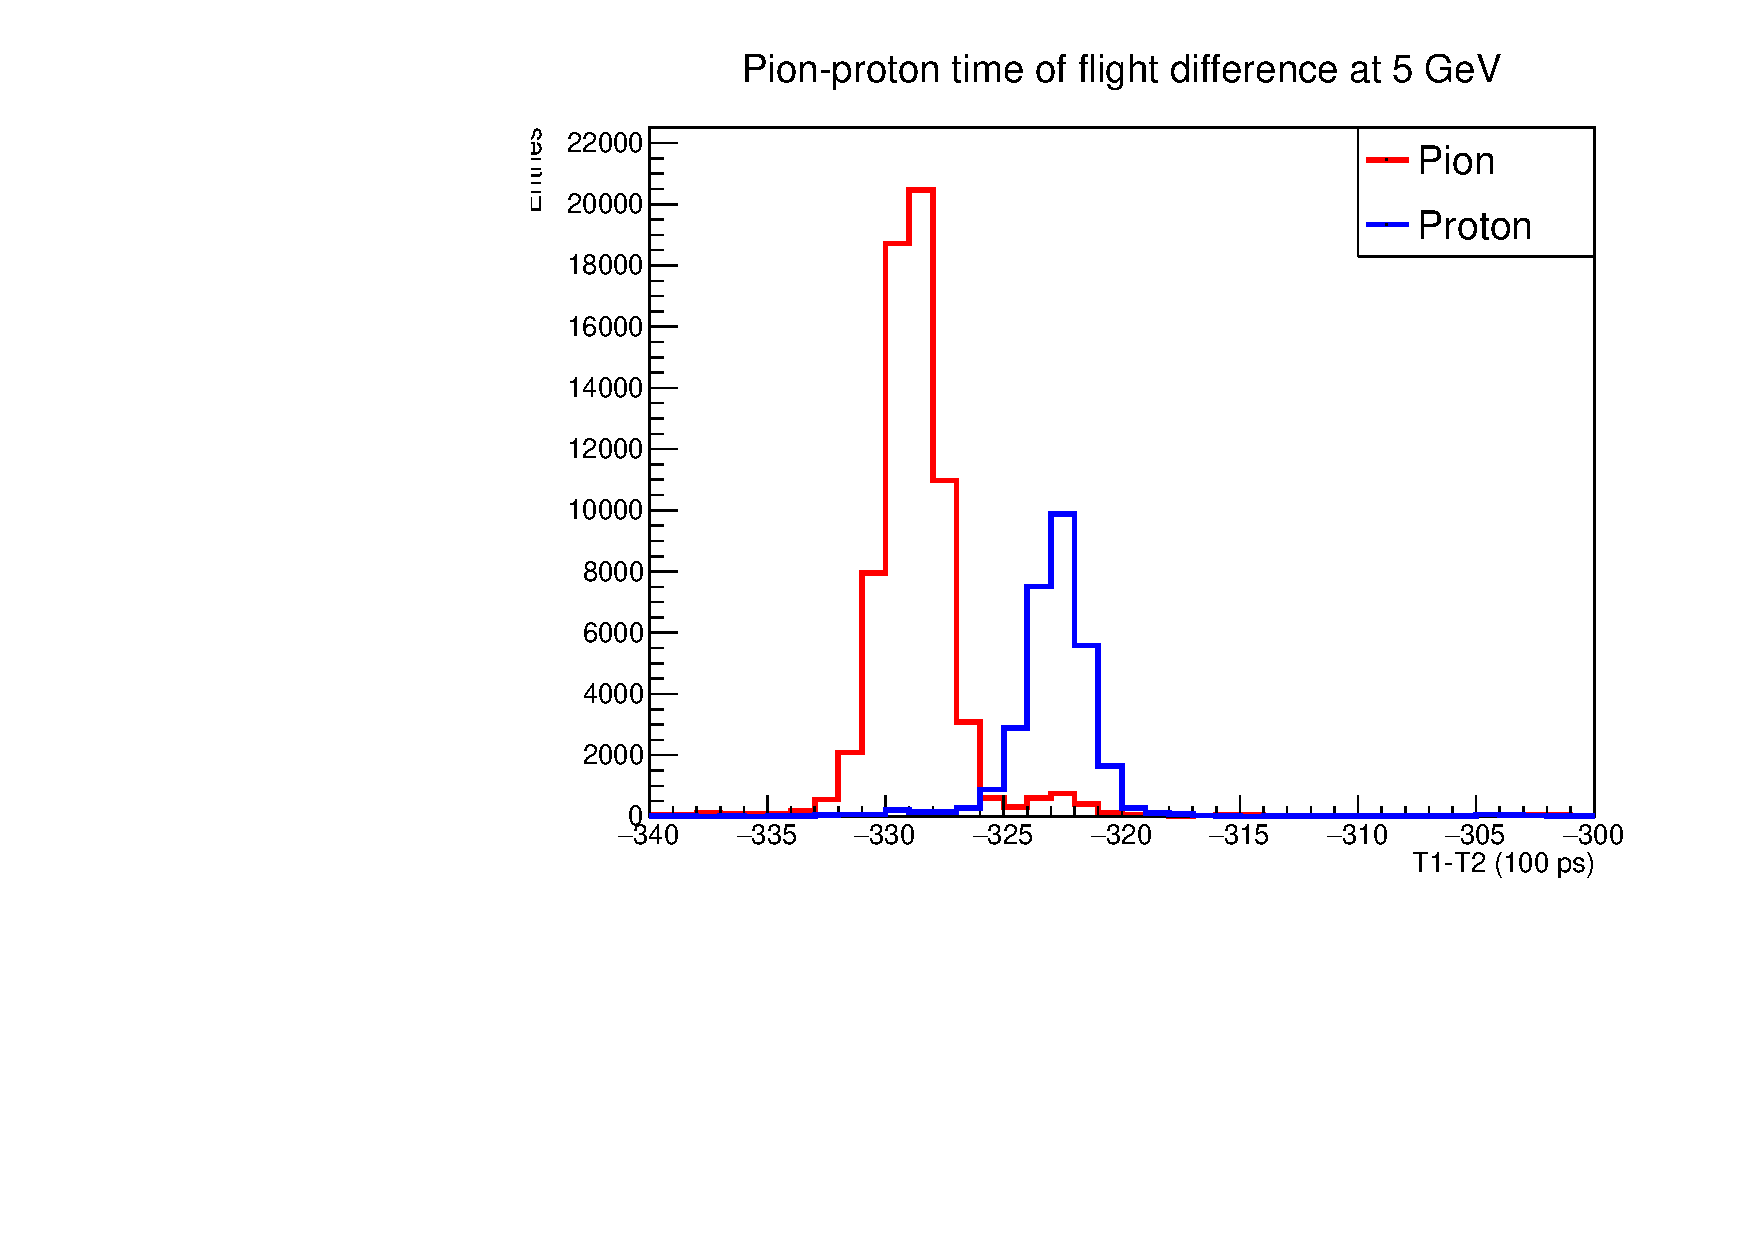
\includegraphics[width = 0.7\textwidth]{Figs/PionProton_TimeDiff_5GeV.pdf}
  \end{figure}
\end{frame}

\begin{frame}{2022 test beam analysis}
  \vspace{0.0cm}
  \begin{center}
    {\large Check time of flight between time references}\\
    {\normalsize Expected time difference at $\SI{3}{\giga\eV}$: $\SI{1.6}{\nano\second}$}
  \end{center}
  \begin{figure}
    \centering
    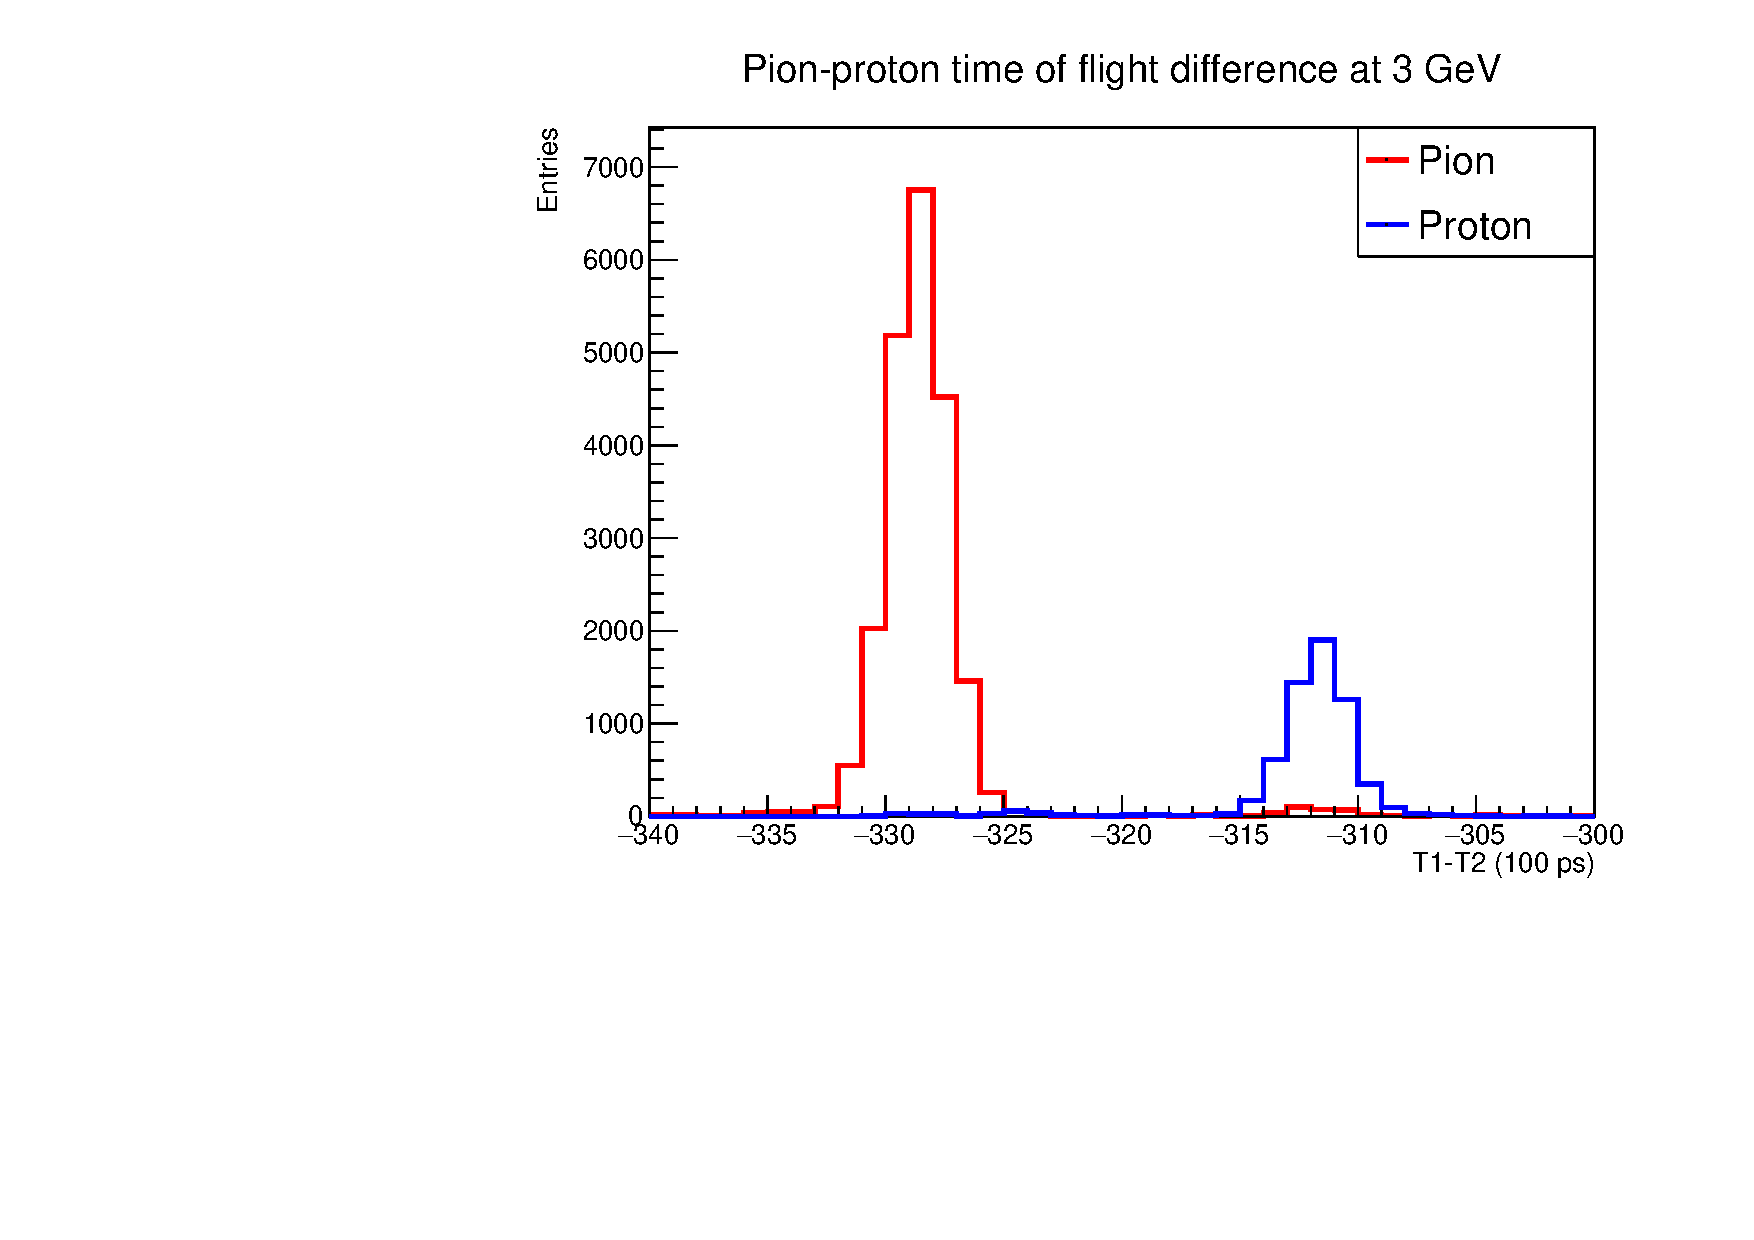
\includegraphics[width = 0.7\textwidth]{Figs/PionProton_TimeDiff_3GeV.pdf}
  \end{figure}
\end{frame}

\begin{frame}{Summary and future prospects}
  \vspace{0.3cm}
  {\Large Summary:}
  \vspace{0.5cm}
  \begin{enumerate}
    \setlength\itemsep{1.5em}
    \item{Test beam analysis progressing well, with promising results}
    \begin{itemize}
      \item{Hit patterns well understood}
      \item{More detailed analysis of time information ongoing}
    \end{itemize}
    \item{We have aquired new electronics and new MCP-PMTs}
    \begin{itemize}
      \item{Lab testing ongoing}
      \item{New electronics will replace legacy NINOs and HPTDCs}
      \item{New MCP-MPTs have higher spatial resolution}
    \end{itemize}
  \end{enumerate}
\end{frame}

\begin{frame}{Summary and future prospects}
  \vspace{0.3cm}
  {\Large Future prospects:}
  \vspace{0.5cm}
  \begin{enumerate}
    \setlength\itemsep{1.5em}
    \item{Finalise test beam analysis}
    \begin{itemize}
      \item{Calibrations}
      \item{Photon counting}
      \item{Time resolution}
      \item{PID performance}
    \end{itemize}
    \item{New test beam is planned for early 2025}
    \begin{itemize}
      \item{Demonstration of full height quartz plate TORCH and mechanics}
    \end{itemize}
  \end{enumerate}
  \vspace{0.5cm}
  \begin{center}
    {\huge Thanks for your attention!}
  \end{center}
\end{frame}

\end{document}
